\documentclass[a4paper,12pt]{article}
\usepackage[english]{babel}
\usepackage[utf8]{inputenc}
\usepackage{graphicx}
\usepackage[titletoc]{appendix}
\usepackage{amsmath}
\usepackage{epstopdf}
\usepackage{pdfpages}
\usepackage{xparse}
\usepackage{kantlipsum}
\usepackage{subcaption}
\usepackage{float}
\usepackage{titlesec}
\usepackage{listings}
\usepackage{courier}
\usepackage{enumitem}
\usepackage{hyperref}
\usepackage{titlesec}
\usepackage[
backend=biber,
style=alphabetic,
sorting=ynt
]{biblatex}
\addbibresource{ref.bib}

\lstset{basicstyle=\footnotesize\ttfamily,breaklines=true}
\graphicspath{ {./images/} }
\usepackage[utf8]{inputenc}
\usepackage[T1]{fontenc}
\usepackage{times}
\usepackage{ifthen}
\usepackage[margin=25mm]{geometry}
\usepackage{fancyhdr}
\pagestyle{fancy}
\setlength{\parindent}{0pt}
\setlength{\parskip}{1ex plus 0.5ex minus 0.2ex}
\newcommand{\twodigit}[1]{\ifthenelse{#1<10}{0}{}{#1}}
\newcommand{\dagensdatum}{\number\year-\twodigit{\number\month}-\twodigit{\number\day}}

%% ------------------------------------------
% NYBILD
% Skapar centrerad bild med caption
%
% #1: Filens url relativt '/images/'
% #2: Caption
% #3: Label
% #4: Skalning
%% ------------------------------------------
\newcommand{\nyBild}[4]{
    \begin{figure}[H]
        \centering
        \includegraphics[angle=0,scale=#4]{images/#1}
        \caption{#2}
        \label{fig:#3}
    \end{figure}
}

%%  Redefinitions of commands containing @
\makeatletter
\makeatother

\newcommand{\LIPStitelsida}{
    {\ }\vspace{45mm}
    \begin{center}
        \textbf{\Huge \LIPSdokumenttyp}
    \end{center}
    \begin{center}
        {\large Alexander Vevstad, Amanda Aasa, Amanda Svennblad, \\Daniel Thomas, Lina Larsson, Olav Berg}
    \end{center}
    \begin{center}
        {\large \textbf{Version \LIPSversion}}
    \end{center}
    \begin{center}
        {Parts of chapter \ref{ch:intro} and \ref{ch:install} are based on the 2019 user guide for ENVISIoN.}
    \end{center}
    \vfill
    \begin{center}{
        \large Status}\\[1.5ex]
        \begin{tabular}{|*{3}{p{40mm}|}}
            \hline
            Granskad & \LIPSgranskare & \LIPSgranskatdatum \\
            \hline
            Godkänd & \LIPSgodkannare & \LIPSgodkantdatum \\
            \hline
        \end{tabular}
    \end{center}
}


\newenvironment{LIPSdokumenthistorik}{
    \begin{center}
        Document history\\[1ex]
        \begin{small}
            \begin{tabular}{|l|l|p{60mm}|l|l|}
                \hline
                \textbf{Version} & \textbf{Date} & \textbf{Changes} &
                \textbf{Done by} & \textbf{Reviewed} \\
                }
                {
                \hline
            \end{tabular}
        \end{small}
    \end{center}
}


\newcommand{\LIPSversionsinfo}[5]{\hline {#1} & {#2} & {#3} & {#4} & {#5} \\}
\newcounter{LIPSkravnummer}
\newcounter{LIPSunderkravnummer}[LIPSkravnummer]

\newenvironment{LIPSkravlista}{
    \begin{tabular}{|p{25mm}|p{25mm}|p{85mm}|p{5mm}|}
        }
        {
        \hline
    \end{tabular}
}

\newenvironment{LIPSleveranslista}{
    \begin{tabular}{|p{25mm}|p{15mm}|p{70mm}|p{25mm}|p{5mm}|}
        }
        {
        \hline
    \end{tabular}
}

\newenvironment{tabellexlista}{
    \begin{tabular}{|p{25mm}|p{25mm}|p{70mm}|p{20mm}|}
        }
        {
        \hline
    \end{tabular}
}

\newenvironment{dokumentlista}{
    \begin{tabular}{|p{28mm}|p{17mm}|p{39mm}|p{28mm}|p{28mm}|}
        }
        {
        \hline
    \end{tabular}
}

\newcommand{\dokumenttext}[5]{
    \hline 
    {#1} & {#2} & {#3} & {#4} & {#5} \\
}


\newcommand{\LIPSkrav}[3]{
    \hline
    \stepcounter{LIPSkravnummer}
    \textbf{Krav nr \arabic{LIPSkravnummer}} & \textbf{{#1}} & {#2} & \textbf{{#3}} \\
}

\newcommand{\tabellex}[3]{
    \hline
    Krav nr x & {#1} & {#2} & {#3} \\
}

\newcommand{\LIPSleverans}[2]{
  {#1} & {#2} & \hline
}

\newcommand{\LIPSunderkrav}[3]{
    \hline\stepcounter{LIPSunderkravnummer}\textbf{Krav nr \arabic{LIPSkravnummer}\Alph{LIPSunderkravnummer}} & \textbf{{#1}} & {#2} & \textbf{{#3}} \\
}

\newenvironment{LIPSprojektidentitet}{%
{\ }\vspace{45mm}
\begin{center}
  {\Large PROJECT IDENTITY}\\[0.5ex]
  {\small
  \LIPSartaltermin, \LIPSprojektgrupp\\
  Faculty of Science and Engineering, Linköping University, IFM
  }
\end{center}
\begin{center}
  {\small Group members}\\
%  \begin{tabular}{|p{30mm}|p{40mm}|p{35mm}|p{45mm}|}
  \begin{tabular}{|l|p{45mm}|p{25mm}|l|}
    \hline
    \textbf{Name} & \textbf{Role} & \textbf{Phone nr.} & \textbf{E-mail} \\
    \hline
}%
{%
    \hline
  \end{tabular}
\end{center}
\begin{center}
  {\small
    \textbf{Website}: \LIPSgrupphemsida\\[1ex]
    \textbf{Client}: \LIPSkund\\
    \textbf{Contact person of client}: \LIPSkundkontakt\\
    \textbf{Course examintor}: \LIPSkursansvarig\\
    \textbf{Main supervisor}: \LIPShandledare\\
  }
\end{center}
\newpage
}
\newcommand{\LIPSgruppmedlem}[4]{\hline {#1} & {#2} & {#3} & {#4} \\}

\NewDocumentCommand\secpdf{somO{1}m}{
  \clearpage
  \thispagestyle{fancy}
  \addcontentsline{toc}{section}{#3}
  \includepdf[
    pages=#4,
    pagecommand={
      \IfBooleanTF{#1}{
        \section*{#3}}{
        \IfNoValueTF{#2}{
          \section{#3}}{
          \section[#2]{#3}}}},
    scale=.80
    ]
    {#5}
}

\newenvironment{LIPSlicens}{
    \begin{center}
    \large{Licens}
    \end{center}
}{}


\usepackage{fancyhdr}
\pagestyle{fancy}
\newcommand{\LIPSdokumenttyp}{USER GUIDE}
\newcommand{\LIPSprojektgrupp}{}
\newcommand{\LIPSversion}{1.0}
\newcommand{\LIPSdatum}{\dagensdatum}
\newcommand{\LIPSartaltermin}{2020/Spring semester}
\newcommand{\LIPSkursnamn}{TFYA75}
\newcommand{\LIPSprojekttitel}{Visualisation of electron structures}
\newcommand{\LIPSgranskare}{}
\newcommand{\LIPSgranskatdatum}{}
\newcommand{\LIPSgodkannare}{}
\newcommand{\LIPSgodkantdatum}{}

\lhead{}
\chead{\textbf{\LIPSprojekttitel}}
\rhead{\textbf{\textsl{LiTH}}\\\textbf{\dagensdatum}}
\lfoot{\textbf{User guide}}
\cfoot{\textbf{\thepage}}
\rfoot{\textbf{\LIPSkursnamn}}

\setlength{\parindent}{0pt}
\setlength{\parskip}{1ex plus 0.5ex minus 0.2ex}

\begin{document}
    \pagenumbering{gobble}
    \LIPStitelsida
    \newpage
    \pagenumbering{roman}
    \newcommand{\LIPSgruppepost}{finns ej}
\newcommand{\LIPSgrupphemsida}{https://liuonline.sharepoint.com/sites/TFYA75/TFYA75\_2019VT\_7Z/62340}

\newcommand{\LIPSdokumentansvarig}{Abdullatif Ismail}
\newcommand{\LIPSkund}{Rickard Armiento, IFM, Linköpings universitet, 581\ 83 Linköping}
\newcommand{\LIPSkundkontakt}{Rickard Armiento, rickard.armiento@liu.se}
\newcommand{\LIPSkursansvarig}{Per Sandström, per.sandstrom@liu.se}
\newcommand{\LIPShandledare}{Johan Jönsson, johan.jonsson@liu.se}

%% Argument till \LIPSgruppmedlem: namn, roll i gruppen, telefonnummer, epost
\begin{LIPSprojektidentitet}
  \LIPSgruppmedlem{Linda Le}{Project leader (PL)}{076-2249926}{linle336@student.liu.se}
  \LIPSgruppmedlem{\LIPSdokumentansvarig}{Document manager(DOK)}{072-0355455}{abdis077@student.liu.se}
  \LIPSgruppmedlem{Anton Hjert}{Anton Hjert (AH)}{070-5728891}{anthj975@student.liu.se}
  \LIPSgruppmedlem{Jesper Ericsson}{Jesper Ericsson (JE)}{070-8772630}{jeser991@student.liu.se}
  \LIPSgruppmedlem{Lloyd Kizito}{Lloyd Kizito (LK)}{070-8230589}{lloki004@student.liu.se}
\end{LIPSprojektidentitet}
    \newpage
    \tableofcontents{}
    \newpage
    %% Argument till \LIPSversionsinfo: versionsnummer, datum, ändringar, utfört av, granskat av
\addcontentsline{toc}{section}{Document history}
\begin{LIPSdokumenthistorik}
  \LIPSversionsinfo{0.1}{2019-05-21}{First draft.}{DOK, AH, JE}{Projektgruppen}
  \LIPSversionsinfo{1.0}{2019-05-25}{Second draft. Rewritten based on comments from the client.}{DOK, AH, JE}{}
\end{LIPSdokumenthistorik}
    \newpage
    \addcontentsline{toc}{section}{Licens}
\begin{LIPSlicens}
    2019 års modifikationer av den tekniska dokumentationen är licensierade under BSD, se bilaga~\ref{ref:licens}. 
\end{LIPSlicens}

    \newpage
    \pagenumbering{arabic}
    \section{Introduction}
\label{ch:intro}
ENVISIoN is an open source toolkit for electron visualization, developed as a part of the course TFYA75: Applied Physics - Bachelor's Project, given at Linköping University, LiU. It's implemented by using a modified verision of the Inviwo visualization framework, developed at the Scientific Visualization Group at Linköping University, LiU.

The present version was developed during the spring semester of 2021 by a project group consisting of: Gabriel Anderberg, Adam Engman, Joakim Stenborg, Kristoffer Gubberud Maras and Didrik Axén. The Supervisor was Marian Brännvall, the Requisitioner and co-supervisor was Rickard Armiento and the Visualisation expert was Peter Steneteg. The Course examiner was Per Sandström. The work is based on a previous version by the project group taking the course in the spring semester of 2020 consisting of: Alexander Vevstad, Amanda Aasa, Amanda Svennblad, Daniel Thomas, Lina Larsson and Olav Berg, with the Supervisor Joel Davidsson, the Requisitioner and co-supervisor Rickard Armiento, the Visualisation expert Peter Steneteg and the Course examiner Per Sandström. That work was based on a previous version by the project group taking the course in the spring semester of 2019 consisting of: Linda Le, Abdullatif Ismail, Anton Hjert, Lloyd Kizito and Jesper Ericsson, with the Supervisor Johan Jönsson, the Requisitioner and co-supervisor Rickard Armiento, the Visualisation expert Peter Steneteg and the Course examiner Per Sandström. That work was based on a previous version by the project group taking the course in the spring semester of 2018 consisting of: Anders Rehult, Marian Brännvall, Andreas Kempe and Viktor Bernholtz with the Supervisor Johan Jönsson, the Requisitioner and co-supervisor Rickard Armiento, the Visualisation expert Rickard Englund and Course examiner Per Sandström. That work was is based on the work by the project group taking the course in the spring term of 2017 consisting of: Josef Adamsson, Robert Cranston, David Hartman, Denise Härnström and Fredrik Segerhammar. Supervisor: Johan Jönsson; Requisitioner and co-supervisor: Rickard Armiento; Visualization expert: Peter Steneteg; and Course examiner: Per Sandström.
\\\\
ENVISIoN provides a graphical user interface and a set of Python scripts that allow the user to:
\begin{itemize}
    \item Read and parse output from electronic structure calculations made by the program VASP and storing the result in a structured HDF5 file.
    
    \item Generate Inviwo visualizations for common tasks when analyzing electronic structure calculations. Presently there is support for visualizing the crystal structure of the unit cell of a material, electron localization function (ELF)-data, electronic charge density, electronic band structure, radial Distribution Function and density of states - both total and partial, forces on atoms as well as molecular dynamics. The system also provides the ability to interconnect some of the networks mentioned above.
\end{itemize}
    \newpage
    \section{How to build Inviwo with ENVISIoN on Ubuntu Linux 20.04}

\label{ch:install}
These instructions show how to build Inviwo and ENVISIoN on Ubuntu Linux 20.04.

\subsection{Install git}
Start by installing git, which will be used to fetch ENVISIoN in the
next step.
\begin{lstlisting}[frame = single, breaklines=true]
    sudo apt install git
\end{lstlisting}

\subsection{Install dependencies}
Install the dependencies for ENVISIoN: 
\begin{lstlisting}[frame = single, breaklines = true]
  sudo apt install \
    python3 python3-pip \
    git \
    python3-numpy python3-h5py python3-pybind11 \
    python3-scipy python3-regex \
    npm
\end{lstlisting}

Install the dependencies for building Inviwo: 
\begin{lstlisting}[frame = single, breaklines = true]
    sudo apt install \
      build-essential gcc-8 g++-8 cmake git freeglut3-dev xorg-dev \
      openexr zlib1g zlib1g-dev \
      qt5-default qttools5-dev qttools5-dev-tools \
      python3 python3-pip \
      libjpeg-dev libtiff-dev libqt5svg5-dev libtirpc-dev libhdf5-dev
      libpng-dev libglu1-mesa-dev libxrandr-dev \
      libxinerama-dev libxcursor-dev
\end{lstlisting}

Check that you have access to Qt 5.12 or later: 
\begin{lstlisting}[frame = single, breaklines = true]
    qmake --version
\end{lstlisting}

If you need to upgrade Qt, you can do the following:
\begin{lstlisting}[frame = single, breaklines = true]
    wget http://download.qt.io/official_releases/qt/5.12/5.12.2/qt-opensource-linux-x64-5.12.2.run
    chmod +x qt-opensource-linux-x64-5.12.2.run
    sudo ./qt-opensource-linux-x64-5.12.2.run
    qtchooser -install opt-qt5.12.2 /opt/Qt5.12.2/5.12.2/gcc_64/bin/qmake
\end{lstlisting}

Check that you have access to cmake 3.12.0 or later by the following command:
\begin{lstlisting}[frame = single, breaklines = true]
    cmake --version
\end{lstlisting}

\subsection{Setup ENVISIoN}
You may build ENVISIoN in whatever directory you want. However, this guide will assume that you build it under your home directory. 

Create a directory under your home directory to build ENVISIoN:

\begin{lstlisting}[frame = single, breaklines=true]
    mkdir ~/ENVISIoN
    cd ~/ENVISIoN
\end{lstlisting}

Download ENVISIoN and install the electron-based gui dependencies:

\begin{lstlisting}[frame = single, breaklines=true]
    git clone https://github.com/rartino/ENVISIoN
    cd ENVISIoN
    npm install
\end{lstlisting}

\subsection{Build Inviwo}
Download and checkout the correct version of the Inviwo source:

\begin{lstlisting}[frame = single, breaklines=true]
    cd ~/ENVISIoN
    git clone https://github.com/inviwo/inviwo
    cd inviwo
    git checkout v0.9.11
\end{lstlisting}

Install the Inviwo submodule dependencies:

\begin{lstlisting}[frame = single, breaklines=true]
    sed -i 's%https://github.com/live-clones/hdf5.git%https://github.com/HDFGroup/hdf5.git%' .gitmodules
    git submodule update --init --recursive
\end{lstlisting}

Apply the ENVISIoN patches to Inviwo:

\begin{lstlisting}[frame = single, breaklines=true]
    git apply \
        "$HOME/ENVISIoN/ENVISIoN/inviwo/patches/deppack_fix.patch" \
        "$HOME/ENVISIoN/ENVISIoN/inviwo/patches/filesystem_env.patch" \
        "$HOME/ENVISIoN/ENVISIoN/inviwo/patches/ftl_fix.patch" \
        "$HOME/ENVISIoN/ENVISIoN/inviwo/patches/transferfunction_extras.patch"
\end{lstlisting}
\newpage
\subsection{Cmake build using system compilers}
Choose the correct Qt version by the following commands:

\begin{lstlisting}[frame = single, breaklines=true]
    qtchooser -l
    export QT_SELECT=<qt version>
    eval `qtchooser --print-env`
\end{lstlisting}

Configure and build Inviwo:

\begin{lstlisting}[frame = single, breaklines=true]
    cd ~/ENVISIoN
    mkdir inviwo-build
    cd inviwo-build/
    cmake -G "Unix Makefiles" \
      -DCMAKE_C_COMPILER="gcc-8" \
      -DCMAKE_CXX_COMPILER="g++-8" \
      -DBUILD_SHARED_LIBS=ON \
      -DIVW_USE_EXTERNAL_IMG=ON \
      -DIVW_EXTERNAL_MODULES="$HOME/ENVISIoN/ENVISIoN/inviwo/modules" \
      -DIVW_MODULE_CRYSTALVISUALIZATION=ON \
      -DIVW_MODULE_GRAPH2D=ON \
      -DIVW_MODULE_HDF5=ON \
      -DIVW_USE_EXTERNAL_HDF5=ON \
      -DIVW_MODULE_PYTHON3=ON \
      -DIVW_MODULE_PYTHON3QT=ON \
      -DIVW_MODULE_QTWIDGETS=ON \
      -DIVW_PACKAGE_PROJECT=ON \
      -DIVW_PACKAGE_INSTALLER=ON \
      -S ../inviwo -B ./
    make -j4
\end{lstlisting}

\emph{Note:}
\begin{itemize}
     \item The number in make -j4 is the number of simultaneous build processes to run. Usually the best choice is the number of CPU cores in your build system.
     \item If you are running into build errors, re-run make with make -j1 to make sure that the last printout pertains to the actual error.
\end{itemize}

\subsection{Verify that the build works correctly}
Start Inviwo to make sure it is built correctly:

\begin{lstlisting}[frame = single, breaklines=true]
    cd ~/ENVISIoN
    inviwo-build/bin/inviwo
\end{lstlisting}

Quit Inviwo and start the ENVISIoN GUI to see that it works:

\begin{lstlisting}[frame = single, breaklines=true]
    cd ~/ENVISIoN/ENVISIoN
    export INVIWO_HOME="$HOME/ENVISIoN/inviwo-build/bin"
    npm start
\end{lstlisting}

\newpage
    \newpage
    \section{How to build Inviwo with ENVISIoN on Windows 10}

These instructions show how to install and build Inviwo and ENVISIoN on Windows 10.

\subsection{Dependencies}
A dependency is a program or software that needs to work because the program you are installing relies on it. To be able to install Inviwo the following dependencies needs to be installed. Inviwo will only compile with Windows 64bit, so make sure all dependencies are also installed as 64bit.

\begin{itemize}
    \setlength\itemsep{0.5em}
    \item \textbf{Anaconda}
    \newline Download [Anaconda]
    \url{https://www.anaconda.com/distribution/#windows} with python 3.7.
    \item \textbf{Qt}
    \newline Download [Qt] (\url{https://www.qt.io/download}) opensource. Version 5.14.2 is tested and recommended. Make sure you select install option MSVC-2017 64-bit.
    \item \textbf{CMake}
    \newline Download and install [Cmake] (\url{https://cmake.org/download/}).
    \item \textbf{Visual Studio 2017}
    \newline Download [Visual Studio 2017] (\url{https://visualstudio.microsoft.com/vs/older-downloads/}). So far, Inviwo has not been able o compile with Visual Studio 2019.
\end{itemize}

\subsection{Setup project}
Open the Anaconda Prompt from your Windows searchbar. Then install the following dependencies by writing this in your prompt:

\begin{lstlisting}[frame = single, breaklines=true]
    conda install git pybind11 numpy scipy matplotlib markdown regex wxpython h5py hdf5 libpng libtiff jpeg cmake nodejs
\end{lstlisting}

Then navigate to your home directory and run the following commands:

\begin{lstlisting}[frame = single, breaklines=true]
    mkdir ENVISIoN
    cd ENVISIoN
\end{lstlisting}

Then you are going to clone Envision when standing in the ENVISIoN directory by running this command:

\begin{lstlisting}[frame = single, breaklines=true]
    git clone https://github.com/rartino/envision
\end{lstlisting}

Next step is to clone Inviwo. Run the following command while still in the ENVISIoN directory:
\begin{lstlisting}[frame = single, breaklines=true]
    git clone https://github.com/inviwo/inviwo
\end{lstlisting}

Then go to the inviwo directory, switch to the branch v0.9.10 and update the registered submodules by running the following commands:

\begin{lstlisting}[frame = single, breaklines=true]
    cd inviwo
    git checkout v0.9.11
    git submodule update --init --recursive
\end{lstlisting}

After this we want to patch Inviwo. Make sure you are in the inviwo directory and run:
\begin{lstlisting}[frame = single, breaklines=true]
    git apply ../ENVISIoN/inviwo/patches/2019/transferfunctionFix.patch
    git apply ../ENVISIoN/inviwo/patches/2019/deb-package.patch
    git apply ../ENVISIoN/inviwo/patches/2019/paneProperty2019.patch
    git apply ../ENVISIoN/inviwo/patches/2019/sysmacro.patch
    git apply ../ENVISIoN/inviwo/patches/2019/inviwo-v0.9.10-extlibs.patch
\end{lstlisting}

\subsection{CMake compiling}
Create a build directory in the ENVISIoN folder that you made earlier. To do this make sure you are standing in the ENVISIoN directory and write:

\begin{lstlisting}[frame = single, breaklines=true]
    mkdir inviwo-build
\end{lstlisting}

Then, open CMake (cmake-gui) and configure the projet with Inviwo as your source code and the new build directory inviwo-build as where to build the binaries. When configuring the project, make sure you select Visual Studio 2017 with x64 for platform option.

The following flags should be added to the default:
\begin{lstlisting}[frame = single, breaklines=true]
    IVW_USE_EXTERNAL_HDF5:BOOL=OFF
    IVW_IMG_USE_EXTERNAL:BOOL=ON
    IVW_EXTERNAL_MODULES:PATH="{path to project}/ENVISIoN/inviwo/modules"
    IVW_MODULE_CRYSTALVISUALIZATION:BOOL=ON
    IVW_MODULE_FERMI:BOOL=ON
    IVW_MODULE_GRAPH2D:BOOL=ON
    IVW_MODULE_PYTHON3:BOOL=ON
    IVW_MODULE_PYTHON3QT:BOOL=ON
    IVW_MODULE_QTWIDGETS:BOOL=ON
    IVW_MODULE_HDF5:BOOL=ON
    IVW_PACKAGE_PROJECT:BOOL=ON
    IVW_PACKAGE_INSTALLER:BOOL=ON
\end{lstlisting}

When done configuring press "Generate" and then open the project with Visual Studio 2017. In Visual Studio, set the build type in the upper menu bar to RelWithDebInfo and make sure that the solution platform is x64. Then press f5 (or fn + f5) and the building of the project should start. This can take some time. Check the Error List during the building to make sure nothing goes wrong. When the building is complete Inviwo should start.

\subsection{Start ENVISIoN}
Go back to your Anaconda Prompt and move to your projects directory (should be ENVISIoN) and run:

\begin{lstlisting}[frame = single, breaklines=true]
    cd ENVISIoN
    npm install
    npm run start
\end{lstlisting}

Now Envision should start and the Envision GUI should pop up. For more information abut how to use ENVISIoN's GUI, see section \ref{sec:GUI}. If you run into errors during the installation, see section \ref{sec:Common errors} where some common errors are listed.


    \newpage
    \section{Preparing VASP-files before starting ENVISIoN}
Before visualizations can be made of input data from VASP, the user have to make sure that VASP-files are made in correct format. This applies to a couple main files in VASP that the user has specified before their VASP-run and also after their VASP-run. The restrictions on the formating of VASP-files are a byproduct of the fact that ENVISIoN has a couple limitations in it's parsing of VASP-files. These limitations are by no way intentional and they are born from theoretical sources and from the time-restrictive nature of the project development itself. 
\subsection{Preparing for bandstructure visualization}

Before deciding to do any visualization of bandstructures at all, be sure that the VASP-files OUTCAR and KPOINTS are available in the VASP-directory you wish to visualize from. Bandstructure visualization can only be made for eight types of brillouin zones if the user wishes to do so. Namely the following: Primitive Cubic (CUB), Body-Centered Cubic (BCC), Face-Centered Cubic (FCC), Primitive Tetragonal (TET), Primitive Hexagonal (HEX), Primitive Orthorhombic (ORC), Primitive Triclinic type 1a/2a (TRI1a/TRI2a) and Primitive Triclinic type 1b/2b (TRI1b/TRI2b). These brillouin zones have fixed symmetry k-points and are specified in an article by Wahyu Setyawan and Stefano Curtarolo \cite{k-points}.

If the user wish to visualize the bandstructure of any other type of brillouin zone, the parser for bandstructures will be unable to interpret the data from VASP. 

Another requirement for a successful visualization of the bandstructure of a brillouin zone type is to format the KPOINTS-file in a specific way such as is illustrated in figure \ref{fig:VASP_band} below. Observe how every two coordinates represents a line between two high-symmetry points as chosen by the $"$line$"$ in the third row, and how each of these pair of coordinates are separated by a blank row for aesthetical reasons. The parser can only handle reciprocal high-symmetry points so make sure that the fourth line in the KPOINTS-file has the word $"$reciprocal$"$ written with no indentation, as shown in the figure.

\begin{figure}[H]
    \centering
    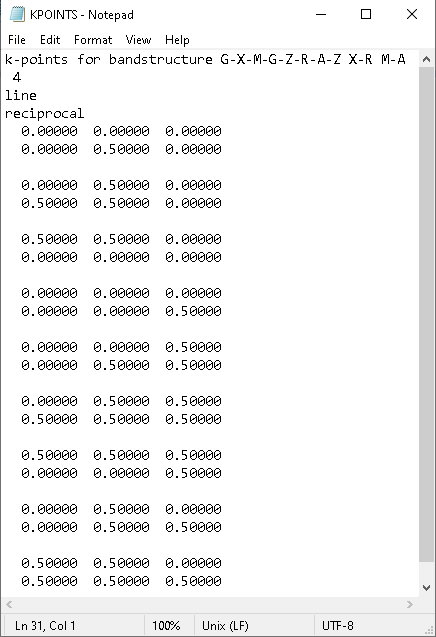
\includegraphics[scale = 0.53]{Images/usermanual_band_TET.png}
    \caption{KPOINTS-file for bandstructure calculation of a TET brillouin zone.}
    \label{fig:VASP_band}
\end{figure}

\subsection{Preparing for fermi-surface visualization}

Make sure that a KPOINTS-file and a EIGENVAL-file is present in the VASP-directory you want to input in ENVISIoN. 

When choosing to visualize fermi-surfaces, make sure that you use the format shown in figure \ref{fig:VASP_fermisurface} for the KPOINTS-file. During visualization of the fermi-surface of a crystal, we want a very big mesh of k-points and an optimal mesh is 10x10x10. Hence make sure that you the fourth row in KPOINTS is at least 10 on each position, as shown in the figure. A very important thing to also note is that the user has to supply the second row with only the a zero, as shown in the figure, as it will force VASP to generate a mesh in the size specified on the fourth row of the file during a VASP-run.

\begin{figure}[H]
    \centering
    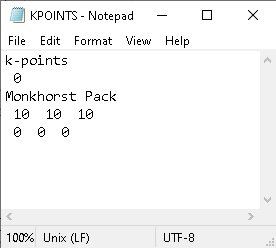
\includegraphics[scale = 0.55]{Images/usermanual_fermisurface.png}
    \caption{KPOINTS-file for fermi-surface visualization.}
    \label{fig:VASP_fermisurface}
\end{figure}

Another, very important, thing to note is that the fermi-surface visualization requires the flag ISYM in the INCAR-file of VASP to be set to the value -1 before a VASP-run. If ISYM is not set to -1, the parser for Fermi-surface will not be able to extrapolate the k-points that are given by VASP, since they are symmetric. If you strive to improve your visualization of the fermi-surface of a crystal, simply increase each integer on the fourth row on the figure above from 10 and above. Observe that the fifth row must have zeroes in order to generate a mesh centered in a origin of the Monkhorst-Pack, without any shifts from this origin. This is for the sake of avoiding errors in the VASP-run.

\subsection{Preparing for unitcell visualization}
\label{section_unit}

Make sure that the VASP-files POTCAR and POSCAR are available in your VASP-directory before you decide to visualize the unitcell. 

For the unitcell visualization, it is very important how you have written the POTCAR-file in relation to the POSCAR-file. Say you have a crystal structure made of three atomic species and you want to do a VASP-run of it. You will first have to find the POTCAR-files for each atomic species, which is supplied by VASP itself. Then you concat them in order to create a single POTCAR-file which represent all atomic species in a single file. Now the dangerous and very common mistake to do in this case is that you concat the separate atomic species POTCARs in an order that does not consist with the order written in the POSCAR-file. This can lead to wrong conclusions of your VASP-calculations. Figure \ref{fig:VASP_unit} examplifies the correct way of concatting POTCARs.

\begin{figure}[H]
    \centering
    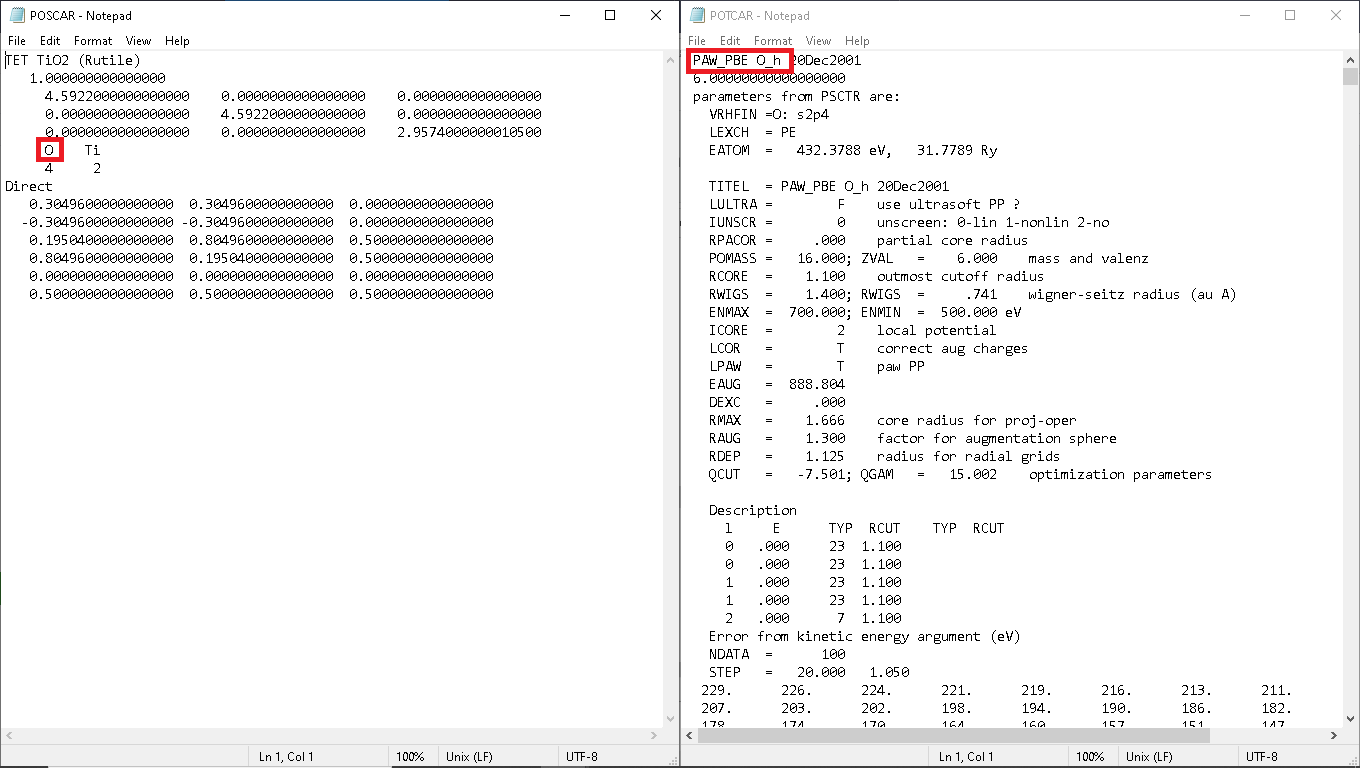
\includegraphics[scale = 0.48]{Images/usermanual_unit_TET.png}
    \caption{In this example with the crystal TiO2, the POSCAR-file has Oxygen written as the first atomic species (red box) and hence the common POTCAR has the pseudopotentials of Oxygen atoms concat first and the pseudopotentials of titanium atoms second.}
    \label{fig:VASP_unit}
\end{figure}

To successfully visualize the unitcell, the user has to make sure that there is no indentation in the row where the user specifies if the atomic positions are given in direct or cartesian coordinates in the POSCAR-file. There is also a requirement that all values in the POSCAR-file, besides the row which supplies the number of atoms per atomic species (which are given in integer form), are given in decimal form (float form). Figure \ref{fig:VASP_unit_1} below shows the correct format of POSCAR in the example with Rutile. Notice how the order of the atomic positions are consistent with the order of the atomic species, which is emphasized by the red box for the O-atom positions and the blue box for the Ti-atom positions.

\begin{figure}[H]
    \centering
    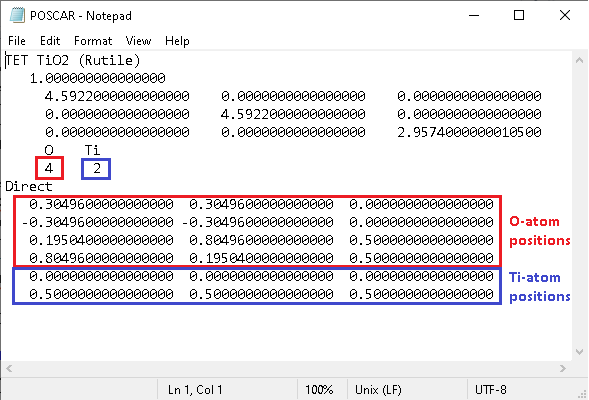
\includegraphics[scale = 0.50]{Images/usermanual_unit_TET_2.png}
    \caption{Example of the correct format of POSCAR-file with the crystal TiO2.}
    \label{fig:VASP_unit_1}
\end{figure}

\subsection{Preparing for DOS visualization}

Make sure that the VASP-files POTCAR, POSCAR, INCAR and DOSCAR are available in your VASP-directory before you decide to visualize the density of states. \\

To ensure an error-free visualization of DOS, follow the directions mentioned in the section \emph{\nameref{section_unit}}, since unitcell data is acquired simultaneously with DOS data with the VASP parser for DOS visualization.

\subsection{Preparing for electron density visualization}

Make sure that the VASP-files POTCAR, POSCAR and CHG are available in your VASP-directory before you decide to visualize the electron density. In the VASP-file INCAR, make sure that LCHARG flag is not set to False, in order to force VASP to write into the CHG-file during the VASP-run. Also make sure that ISYM flag in the VASP-file INCAR is not set to -1 before a VASP-run, which is done for the fermi-surface visualization, as this can cause a wrong visualization of the electron density.\\

To ensure an error-free visualization of electron density, follow the directions mentioned in the section \emph{\nameref{section_unit}}, since unitcell data is acquired simultaneously with electron density data with the VASP parser for electron density visualization.

\subsection{Preparing for force visualization}
Make sure the VASP-files POSCAR and OUTCAR are available in your VASP-directory before visualising force vectors. If these two files are present and in unchanged condition the force vector visualisation should commence non-erroneously.

Notice that in many VASP-directories the forces acting on atoms will be zero, in these cases the vectors will instead be represented as discs in the middle of the atoms, analogous to having a length of zero.

\subsection{Preparing for molecular dynamics visualization}
Make sure that the VASP-files POSCAR, OUTCAR and XDATCAR are available in your VASP-directory before you decide to visualize the molecular dynamics. The IBRION flag has to be set to 0 in the VASP-file OUTCAR for the visualization to run, it's the IBRION flag that decides if  molecular dynamics is possible or not. The NSW flag in the OUTCAR file will be the amount of time steps for the visualization, check if this seems to be correct. \\

The XDATCAR file should contain data for the positions of each atom for all the time steps, if something is wrong with the XDATCAR file the IBRION flag in the OUTCAR flag probably is not set to the correct value for molecular dynamics. From the POSCAR file you will receive data about the elements and the amount of each sort of atom.   

\newpage

\section{Preparing ELK-files before starting ENVISIoN}
Before visualizations can be made of input data from ELK, the user have to make sure that the correct ELK-files are provided and made in the correct format for the visualization that the user wants to run.

\subsection{Preparing for unitcell visualization}

Make sure that the ELK-files INFO.OUT and EQATOMS.OUT are available in your ELK-directory before you decide to visualize the unitcell. If thees two files exist the visualization should be able to run.  

\subsection{Preparing for force visualization}

To run a force visualization task nr 2 must be run when elk performs calculations. Look in the elk.in and confirm that this is done. Make sure the ELK-files INFO.OUT and EQATOMS.OUT are available in your ELK-directory before visualising force vectors. If these two files are present in unchanged condition and task nr 2 has bean preformed the force vector visualisation should commence non-erroneously. If the forces acting on atoms is zero the vectors will instead be represented as discs in the middle of the atoms, analogous to having a length of zero. 

\subsection{Preparing for elf visualization}
To run a elf visualization task nr 53 must be run when elk performs calculations. Look in the elk.in and confirm that this is done. Make sure the ELK-files INFO.OUT and ELF3D.OUT are available in your ELK-directory before visualising elf. If these two files are present in unchanged condition and task nr 53 has bean preformed the elf visualisation should commence non-erroneously.



\newpage


    \section{Start ENVISIoN or Inviwo}
\label{sec: start envision}
\subsection{Start ENVISIoN}
When the building for Inviwo with ENVISIoN is finished, we can start the application's graphical user interface. If you have structured the file system as explained in section 2 and section 3, the start up of the application should be the same on every operating system. Open up a terminal or command window and execute the following command in the terminal:

\begin{lstlisting}[frame = single, breaklines = true]
    python3 ~/ENVISIoN/ENVISIoN/envisionGUI/GUI.py
\end{lstlisting}

The application ENVISIoN should start and the GUI will pop up. For further instruction concering ENVISIoN's GUI, see section \ref{sec:newGUI}.

\subsection{Start Inviwo}
During the development of ENVISIoN it can be an advantage to use only Inviwo and its graphical user interface. If the installation of ENVISIoN with Inviwo is made correctly, open a terminal or command window and navigate to the ENVISIoN directory: 

\begin{lstlisting}[frame = single, breaklines = true]
    cd ~ENVISIoN/ENVISIoN
\end{lstlisting}

Then, type in the following command in the terminal to start Inviwo:

\begin{lstlisting}[frame = single, breaklines = true]
    inviwo-build/bin/inviwo
\end{lstlisting}
    \newpage
    \section{Start Inviwo and run ENVISIoN scripts}

\\
If the user wishes to run Inviwo with its own graphical user interface, it's possible and still have access to the visualizations provided by ENVISIoN. These visualizations are stored in the form of Python scripts that can be compiled through the Inviwo user interface.

To run Inviwo in an UNIX environment, execute the commands below.

\begin{lstlisting}[frame = single, breaklines=true]
    cd ~/ENVISIoN/ENVISIoN
    inviwo-build/bin/inviwo
\end{lstlisting}

When the Inviwo interface has opened, follow the instructions given in figure \ref{fig:Inviwo} and in the list below to run a visualization script.

\begin{enumerate}
\item Locate and press the Python menu in the Inviwo bar.
\item Open the Python editor by pressing it.
\item In the Python editor, click Open Script.
\item Select one of the scripts. The ENVISIoN scripts can be located in \emph{$\sim$/ENVISIoN/demo}.
\item Click open.
\item Click the button in the top left corner to run.
\end{enumerate}

\begin{figure}[ht]
    \centering
    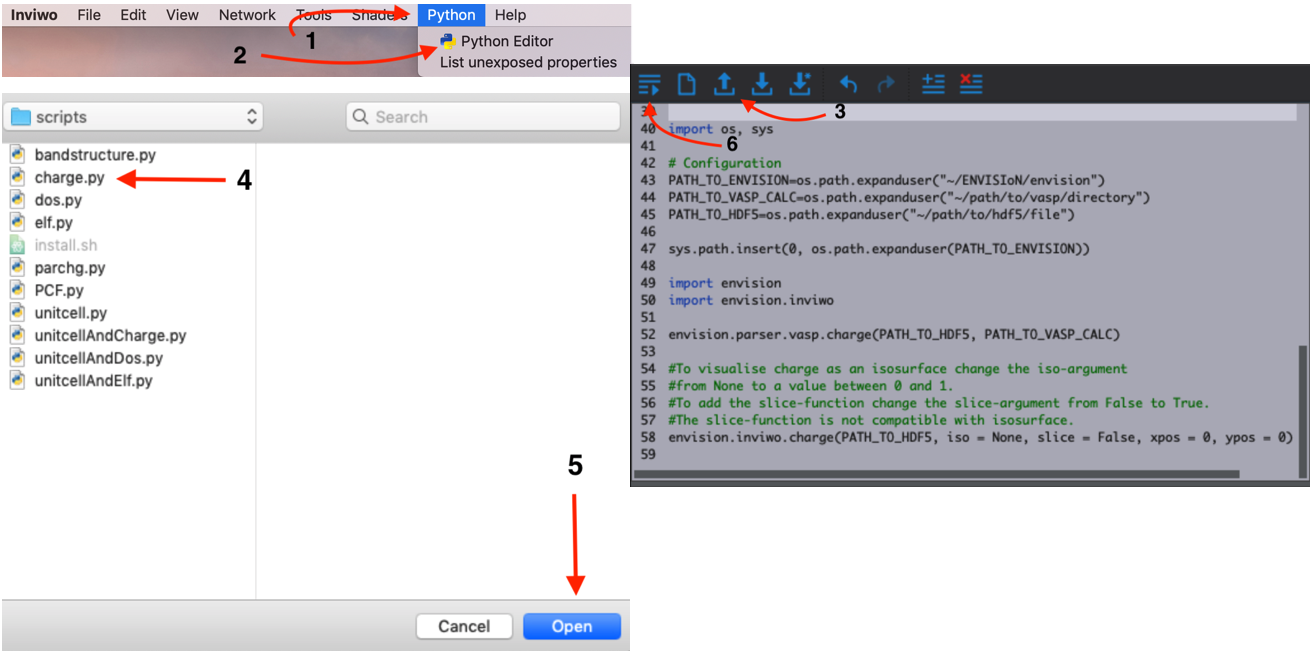
\includegraphics[angle=0, width=\linewidth]{Images/completeInviwo.png}
    \caption{Cutout from Inviwo with instructions on how to run a ENVISIoN visualization script in numeric order.}
    \label{fig:Inviwo}
\end{figure}

    \newpage
    \section{Using Legacy GUI}
\label{sec:GUI}
ENVISIoN is equipped with a graphical user interface to simplify the usage of ENVISIoN. 

\subsection{Start-up}
When the user starts the application through a computer terminal (see chapter \ref{sec: start envision}) a window opens, see figure \ref{fig:GUIStartupUbuntu} for Ubuntu and figure for Windows. The start-up window of ENVISIoN has a sidebar menu to the left with different choices. Each choice has its own content to the right. By default, the ``Dataset loader'', is chosen from start. The other possible choices are ``Parser'' or ``About''. Under ``Active datasets'' the loaded datasets will appear. Each alternative will be explained in their own sections in this chapter. The following figures of the GUI in this chapter will be for Windows but the content is the same for every operative system.

\begin{figure}[H]
    \centering
    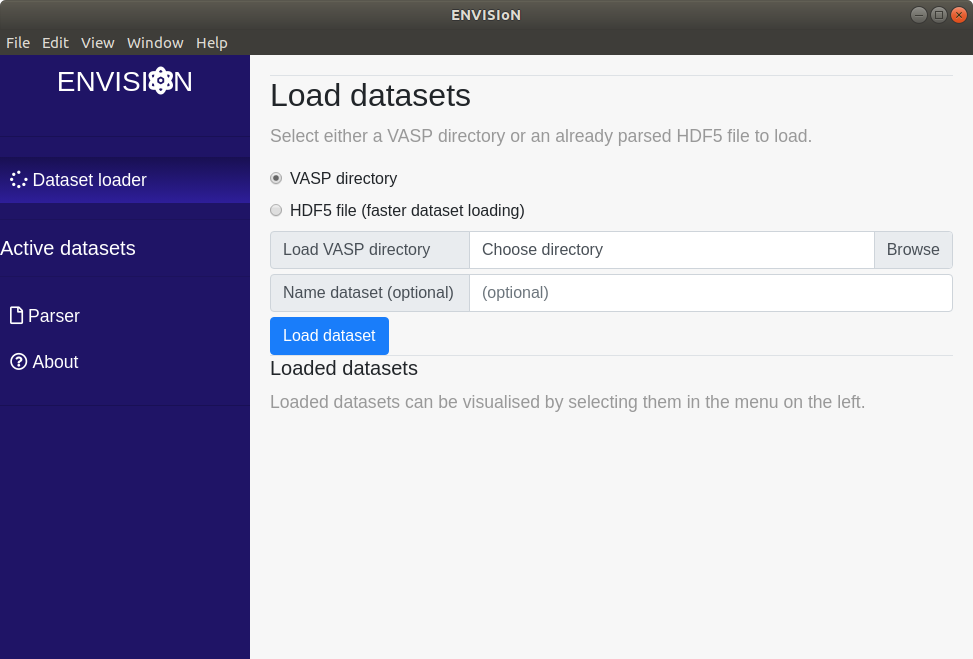
\includegraphics[scale = 0.3]{Images/GUI_start_Ubuntu.png}
    \caption{ENVISIoN start-up window for Linux.}
    \label{fig:GUIStartupUbuntu}
\end{figure}

\begin{figure}[H]
    \centering
    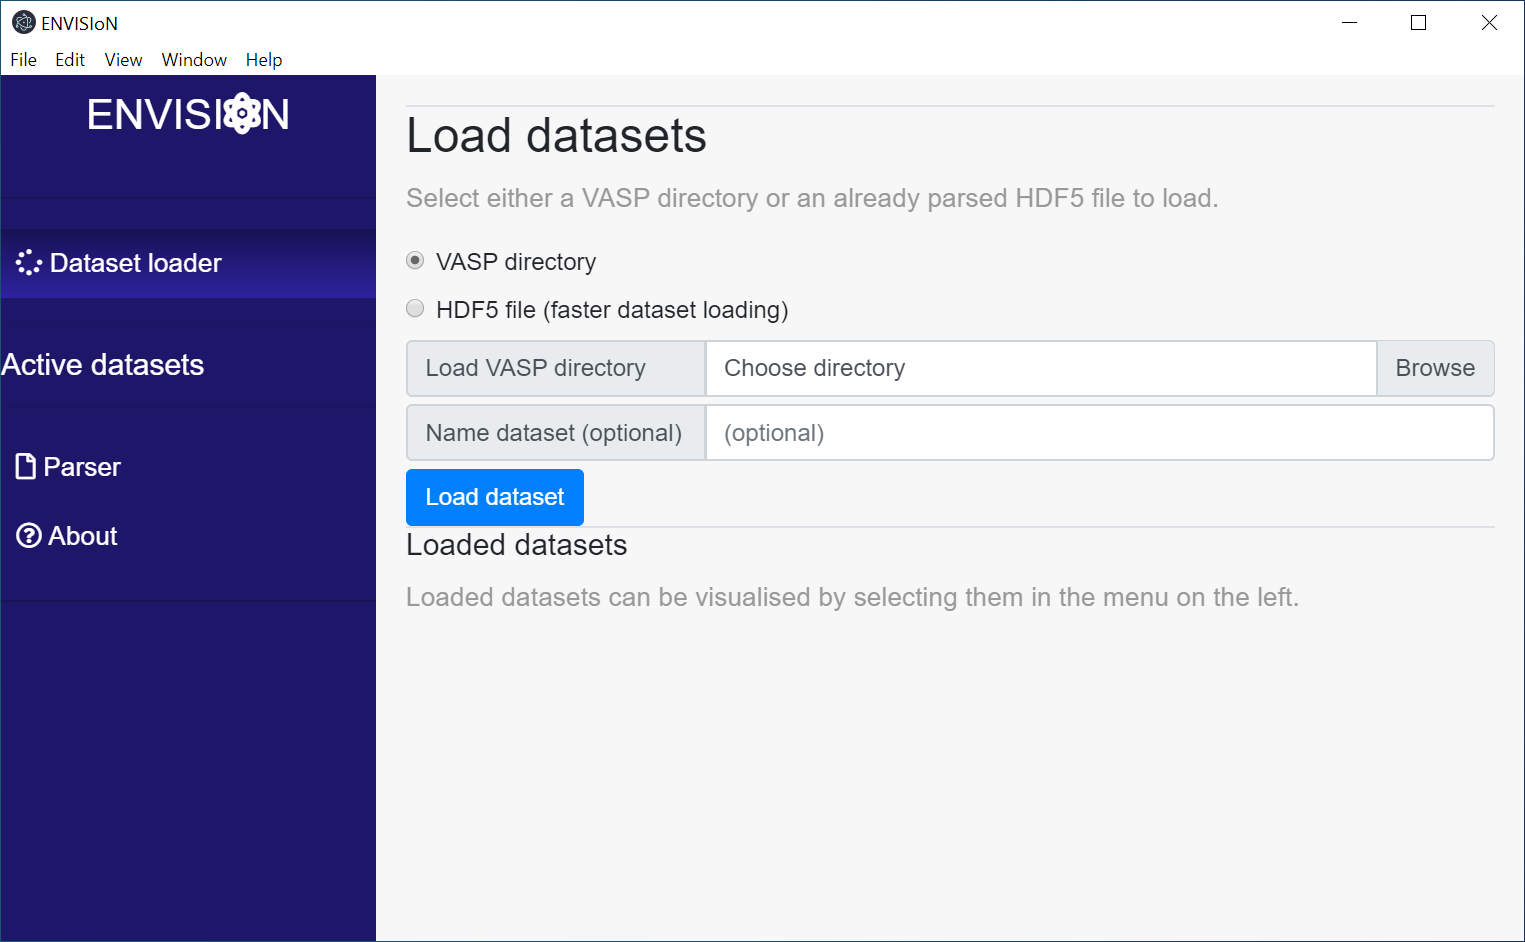
\includegraphics[scale = 0.4]{Images/GUI_start_Windows.png}
    \caption{ENVISIoN start-up window for Windows.}
    \label{fig:GUIStartupUbuntu}
\end{figure}

\subsection{Dataset loader}
In the ``Dataset loader'' a user can select either a VASP file or a HDF5 file to load which then will be visualised. To load a VASP file, the box ``VASP directory'' need to be checked. To load a HDF5 file the box ``HDF5 file'' need to be checked. 

For a quick step-by-step guide, scroll down to section \ref{sec:Dataset step-by-step}.

\subsubsection{Load a VASP file}
For loading a VASP file, the content for the ``Dataset loader'' is shown below in figure \ref{fig:GUIDatasetloaderVASP}.

\begin{figure}[H]
    \centering
    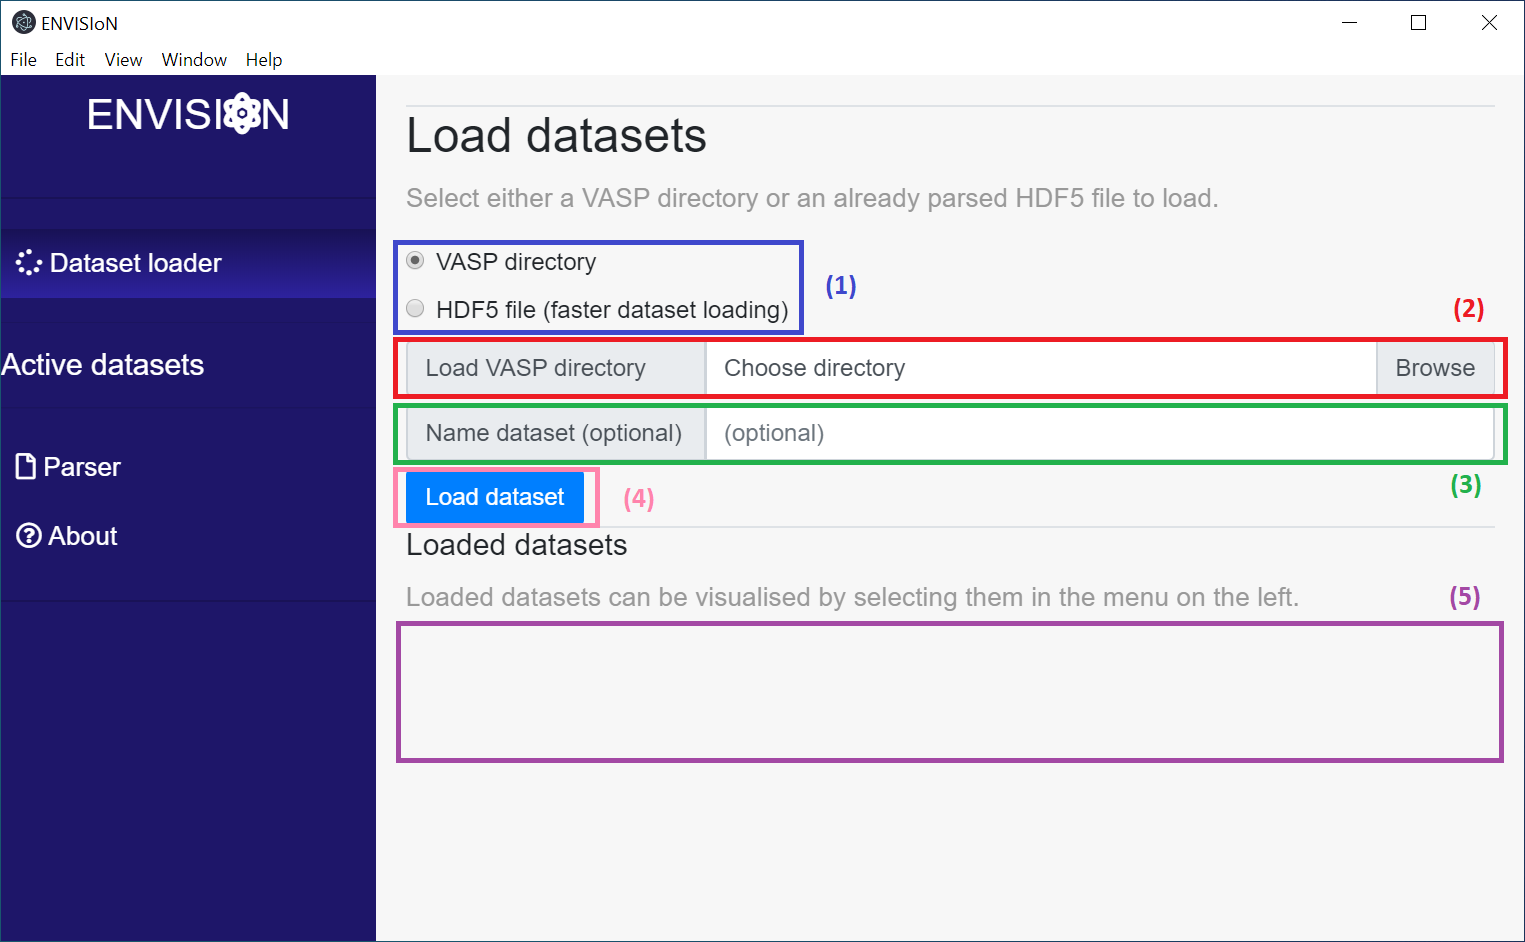
\includegraphics[scale = 0.45]{Images/GUI_Datasetloader_VASP.png}
    \caption{Dataset loader for VASP source.}
    \label{fig:GUIDatasetloaderVASP}
\end{figure}

In the blue box labeled (1) the box ``VASP directory'' need to be checked. In the red box labeled (2) the path to the VASP directory to load is selected. By clicking on ``Browse'' a new window will appear where the user navigates to the VASP directory on the computer and selects it. In the green box labeled (3) the user can write a name for the dataset. This is optional. In the pink box labeled (4) is the ``Load dataset'' button. When pressing this button the dataset will be loaded. The loaded dataset will be displayed in the purple box labeled (5) and in the sidebar menu under ``Active datasets''.

\subsubsection{Load a HDF5 file}
For loading a HDF5 file, the content for the ``Dataset loader'' is shown below in figure \ref{fig:GUIDatasetloaderHDF5}.

\begin{figure}[H]
    \centering
    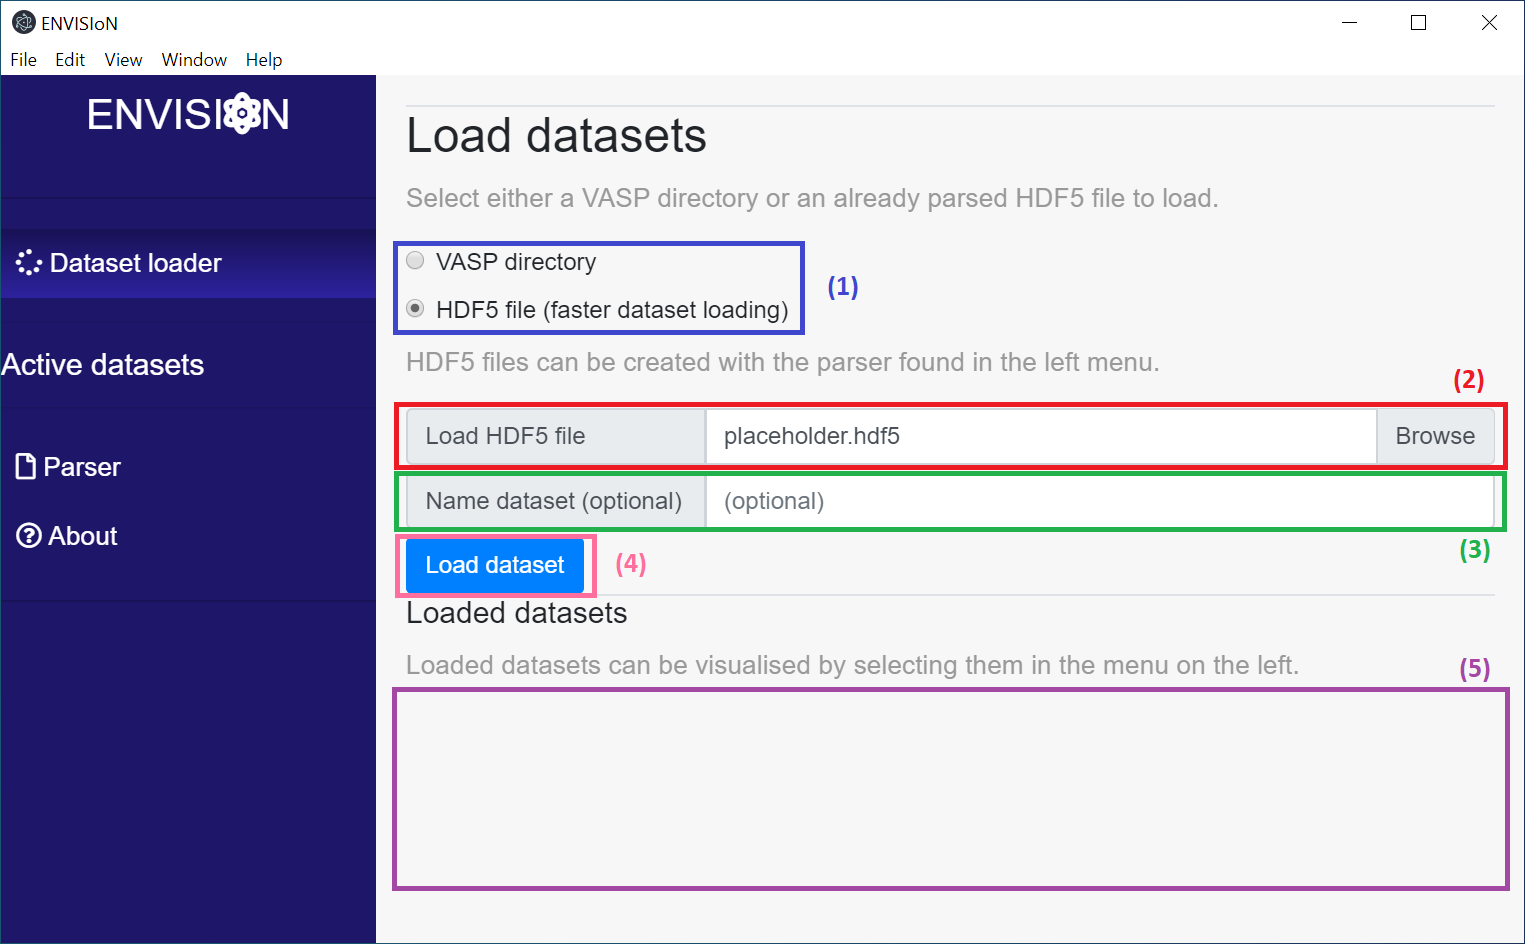
\includegraphics[scale = 0.45]{Images/GUI.Datasetloader_HDF5.png}
    \caption{Dataset loader for HDF5 source.}
    \label{fig:GUIDatasetloaderHDF5}
\end{figure}

In the blue box labeled (1) the box ``HDF5 file'' need to be checked. In the red box labeled (2) the path to the HDF5 file to load is selected. By clicking on ``Browse'' a new window will appear where the user navigates to the HDF5 file on the computer and selects it. In the green box labeled (3) the user can write a name for the dataset. This is optional. In the pink box labeled (4) is the ``Load dataset'' button. When pressing this button the dataset will be loaded. The loaded dataset will be displayed in the purple box labeled (5) and in the sidebar menu under ``Active datasets''.

\subsubsection{Quick Step-by-step guide}
\label{sec:Dataset step-by-step}
To load a VASP-file (referring to figure \ref{fig:GUIDatasetloaderVASP}):
\begin{enumerate}
    \item Check the box ``VASP directory'' in (1).
    \item Choose a VASP directory on your computer by clicking ``Browse'' in (2).
    \item (optional) Name the dataset by writing in (3).
    \item Click ``Load dataset'' in (4).
    \item Now the loaded dataset is showing in (5) and in the sidebar menu under ``Active datasets''.
\end{enumerate}

To load a HDF5 file (referring to figure \ref{fig:GUIDatasetloaderHDF5}):
\begin{enumerate}
    \item Check the box ``HDF5 file'' in (1).
    \item Choose a HDF5 file on your computer by clicking ``Browse'' in (2).
    \item (optional) Name the dataset by writing in (3).
    \item Click ``Load dataset'' in (4).
    \item Now the loaded dataset is showing in (5) and in the sidebar menu under ``Active datasets''.
\end{enumerate}

\subsection{Active datasets}
When a dataset is loaded for visualisation it will appear under ``Active datasets'' in the sidebar menu. 

\subsubsection{Starting the visualisation}
By clicking on one of datasets under ``Active datasets'', new content will show up to the right, see figure \ref{fig:GUIChosevistype} below. In figure \ref{fig:GUIChosevistype} the dataset ``BaSO4\_ORC'' is loaded as an example.

\begin{figure}[H]
    \centering
    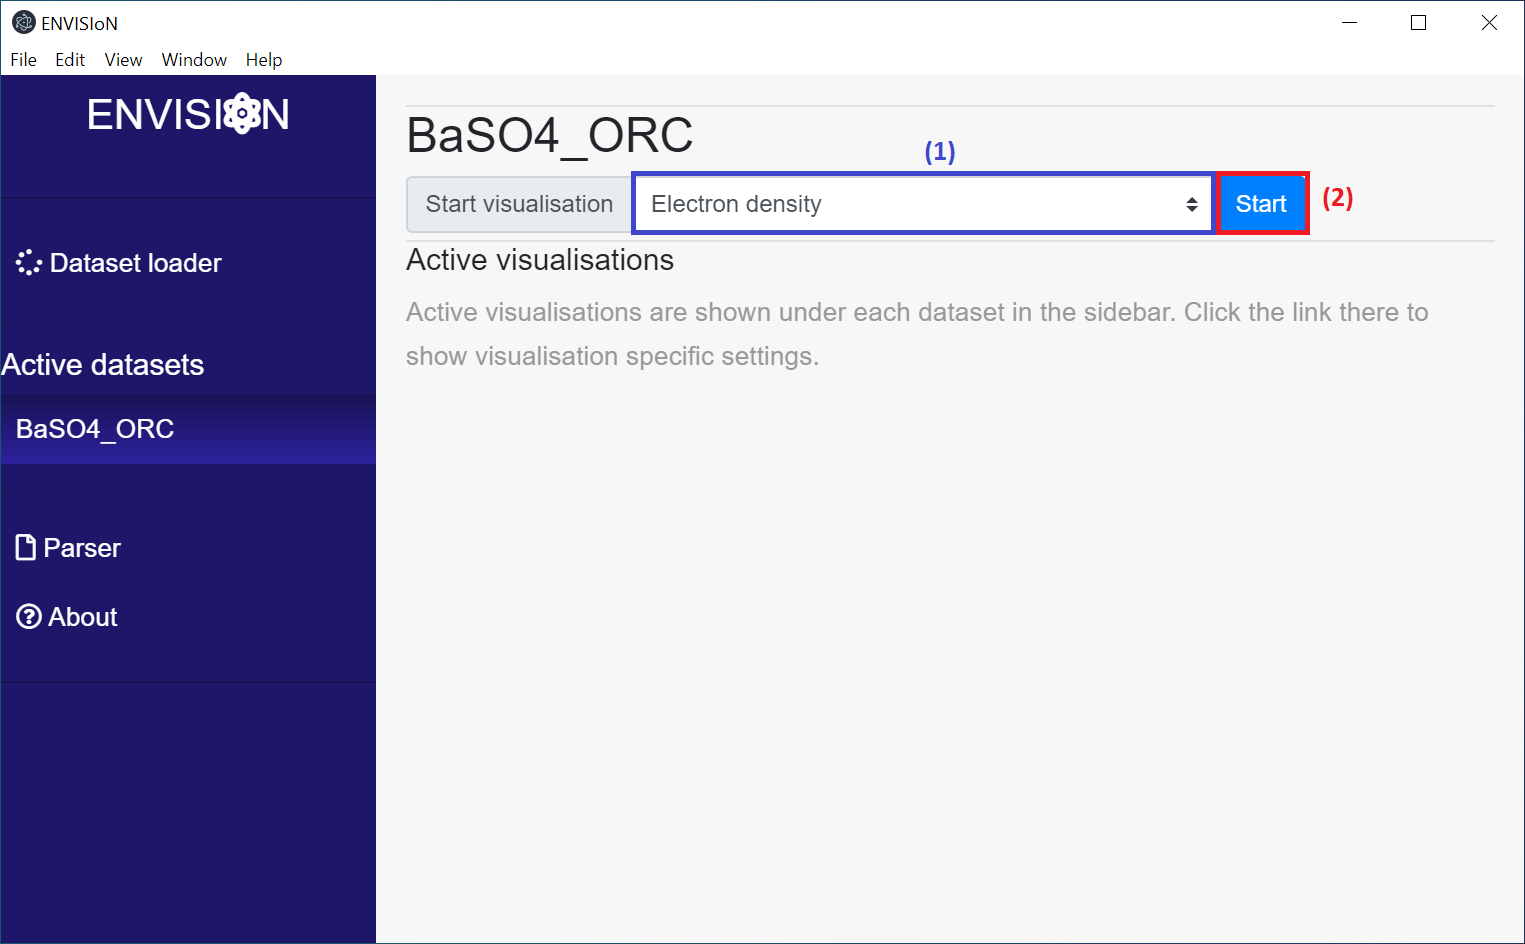
\includegraphics[scale = 0.45]{Images/GUI_Chosevistype.png}
    \caption{Start the visualisation. Here the dataset BaSO4\_ORC is loaded as an example.}
    \label{fig:GUIChosevistype}
\end{figure}

By pressing the area inside the blue box labeled (1) the user can select which visualisation type to visualise from the drop-down menu. The different possible visualisation types are: 

\begin{itemize}
    \item Electron density
    \item Unitcell
    \item Bandstructure 3D
    \item Fermi surface
\end{itemize}

In the red box labeled (2) is the ``Start'' button. When pressing this button the visualisation will start for the chosen visualisation type. The visualisation will appear under the loaded dataset in the sidebar menu. When pressing the visualisation in the sidebar menu new content with visualisation controls will appear to the right. Also the canvas/canvases belonging to the selected visualisation type will pop up next to the GUI.

\subsubsection{Visualisation controls}
When clicking on the ongoing visualisation of a dataset in the sidebar, visualisation controls will appear to the right. These controls are different for different visualisation types. There are only controls for the visualisation types ``Electron density'' and ``Fermi surface''. 

\textbf{Electron density controls}
\newline
If the ongoing visualisation is ``Electron Density'' the controls for interacting with the visualisation are shown in figure \ref{fig:GUICharge} below.

\begin{figure}[H]
    \centering
    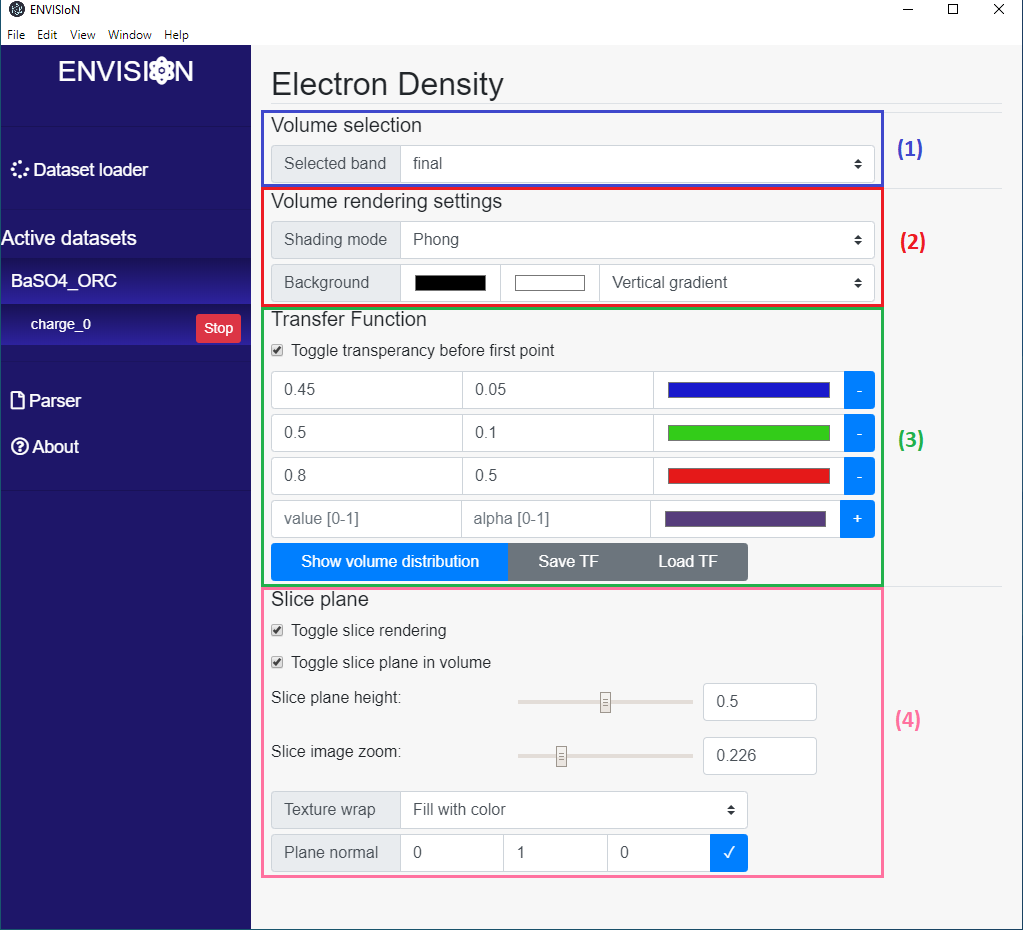
\includegraphics[scale = 0.56]{Images/GUI_Chargecontent.png}
    \caption{The content for the electron density visualisation controls.}
    \label{fig:GUICharge}
\end{figure}

For electron density the user can control the volume selection by selecting band, the volume rendering settings, the transfer function by visualising certain density intervals with different colors and the slice plane to see the electron density in a 2-dimensional plane. In the blue box labeled (1) the user can regulate the volume selection by selecting which band to visualise from a drop-down menu. In the red box labeled (2) the user can select the Shading mode from a drop-down menu and also change the Background color and gradient. In the green box labeled (3) the user can change the transfer function. This is a way to choose different colors for different electron density intervals. The intervals are normalized. The user can also select the blue ``Show volume distribution'' button and then a new diagram will pop up containing information about the volume distribution for the selected dataset. In the pink box labeled (4) the user can configure the slice plan to see a 2-dimensional cross-sectional area of the electron density connected to the 3-dimensional electron density.

\textbf{Fermi surface controls}
\newline
If the ongoing visualisation is ``Fermi surface'' the controls for interacting with the visualisation are shown in figure \ref{fig:GUIFermi} below.

\begin{figure}[H]
    \centering
    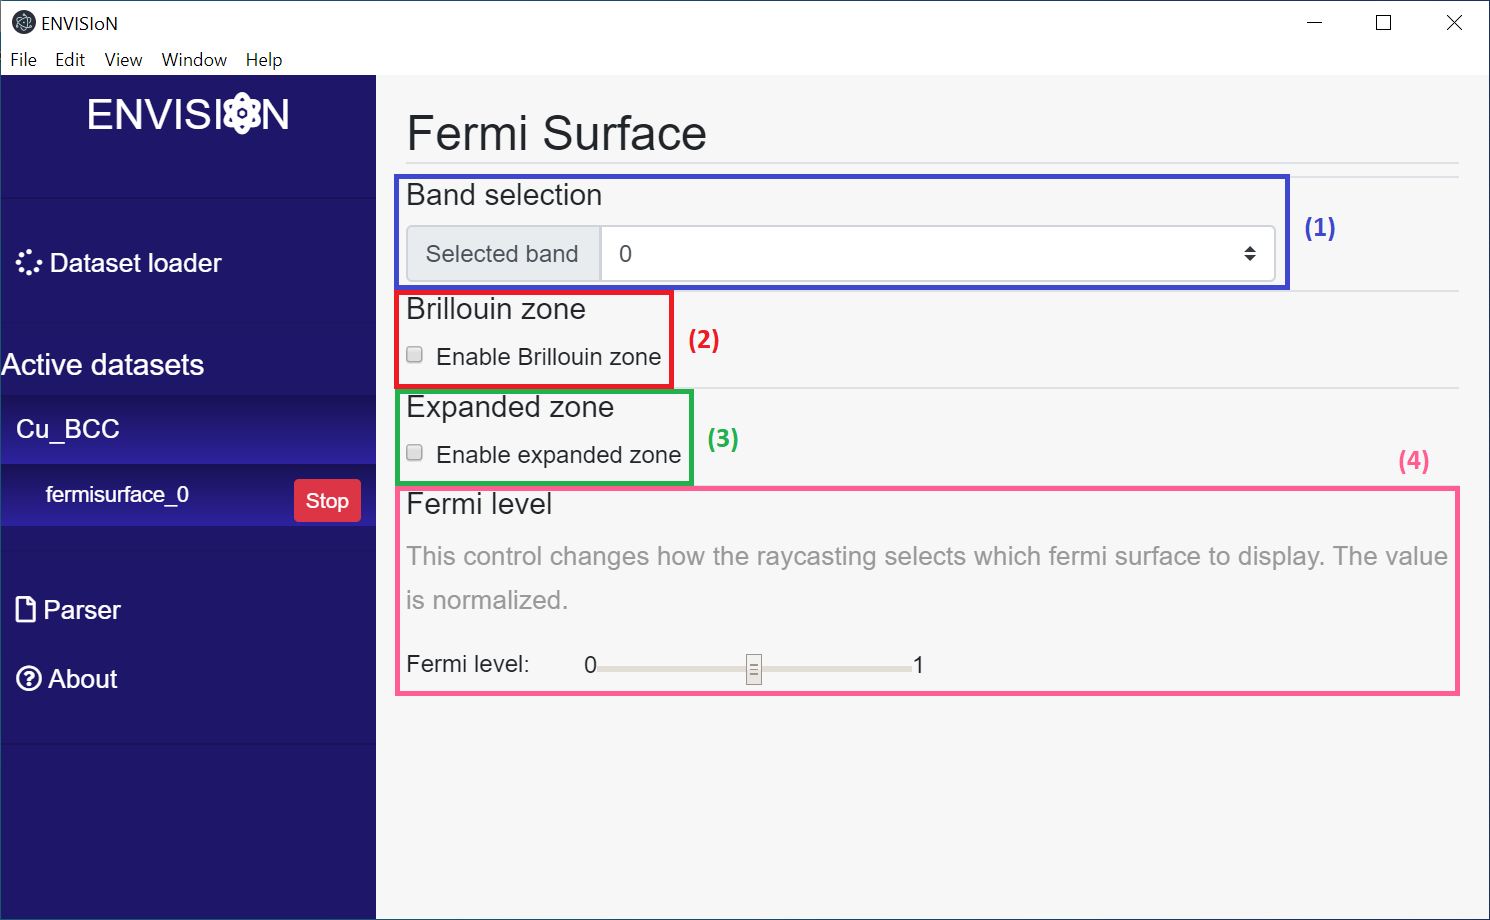
\includegraphics[scale = 0.45]{Images/GUI_Fermicontent.png}
    \caption{The content for the fermi visualisation controls.}
    \label{fig:GUIFermi}
\end{figure}

For fermi surface the user can control which band that should be visualised, enable the Brillouin zone, enable expanded zone and regulate the fermi level. In the blue box labeled (1) the user can select which band to visualise from a drop-down menu. When starting the visualisation the current band will be selected automatically and also the correct fermi level (in the pink box labeled (4)) for each band is set to default. In the red box labeled (2) the user can enable or disable the Brillouin zone by having the checkbox checked or unchecked. In the green box labeled (3) the user can enable or disable expanded zone by having the checkbox checked or unchecked. In the pink box labeled (4) the user can control the fermi level by dragging the slider to the right or to the left. The scale is normalized between 0 and 1.

\subsection{Parser}
If you choose ``Parser'' in the sidebar menu, new content will be exposed to the right, see figure \ref{fig:GUIParser} below. 

\begin{figure}[H]
    \centering
    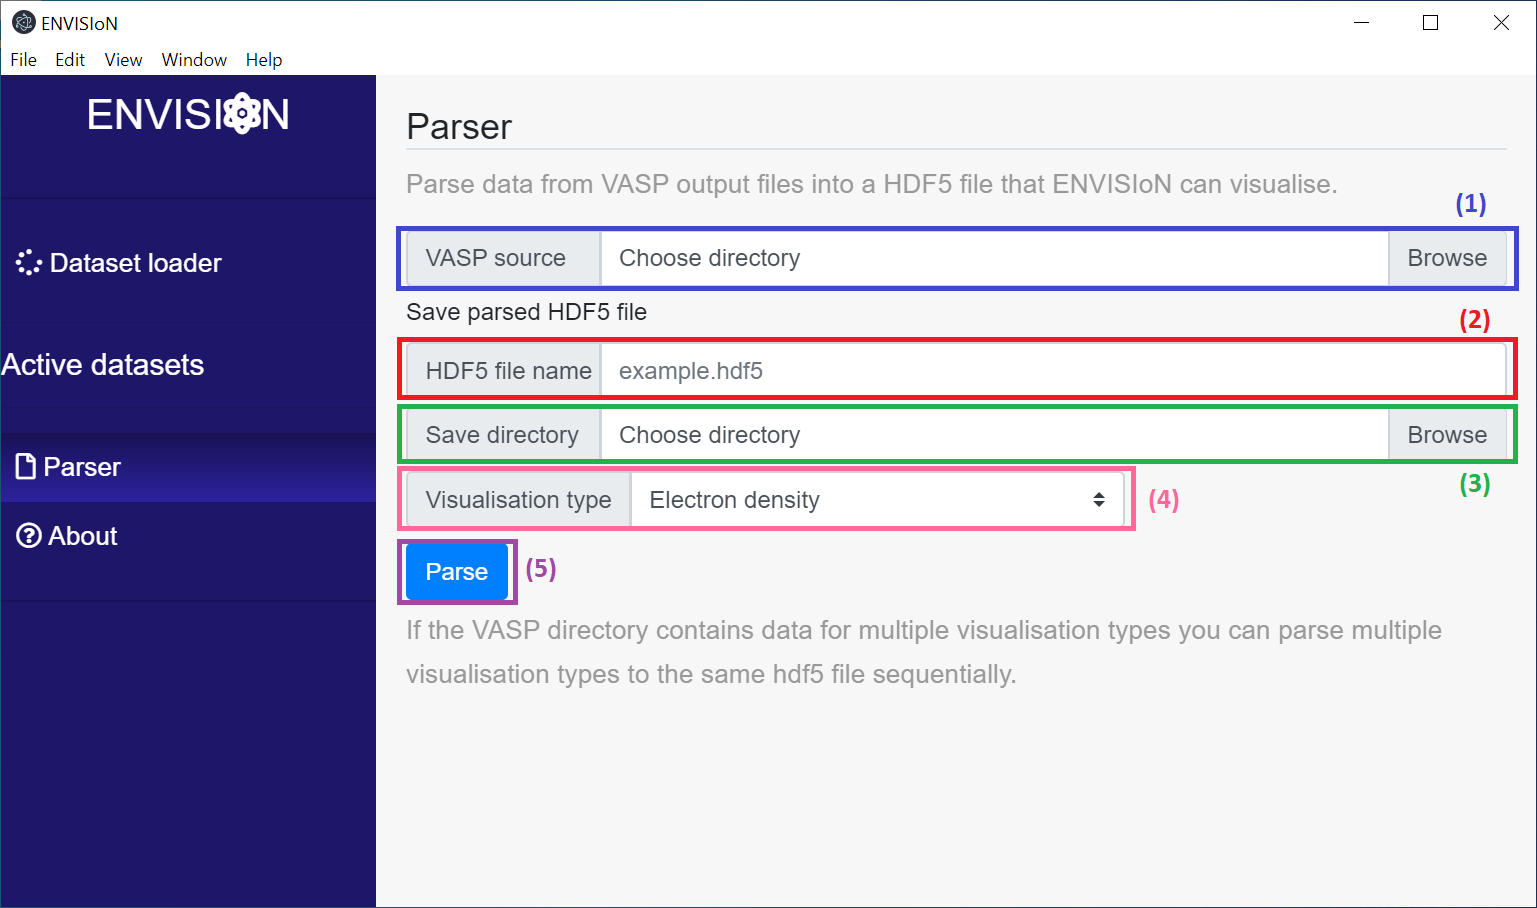
\includegraphics[scale = 0.45]{Images/GUI_Parserstart.png}
    \caption{The content for the parser menu.}
    \label{fig:GUIParser}
\end{figure}

For a quick step-by-step guide, scroll down to section \ref{sec:Parse step-by-step} 

In figure \ref{fig:GUIParser}, in the blue box labeled (1), the path to the directory of VASP files to parse is selected. By clicking on ``Browse'' a new window will appear where the user navigates to the directory of the VASP files on the computer and selects it. In the red box labeled (2) the user writes the name for the new HDF5 file, it needs to end with .hdf5. In the green box labeled (3) the path to the saving directory of the new HDF5 file is selected. When clicking on ``Browse'' a new window will appear where the user navigates to the saving directory and selects it. In the pink box labeled (4) the user can select which visualisation type to parse from a drop-down menu. The possible types to parse are:

\begin{itemize}
    \item Electron density
    \item Bandstructure
    \item Unitcell
    \item Fermi surface
\end{itemize}

In the purple box labeled (5) is the ``Parse'' button. By pressing this button the parser will parse the VASP files and create a HDF5 file in the saving directory. 

\subsubsection{Quick Step-by-step guide}
\label{sec:Parse step-by-step}
Parsing VASP files to a HDF5 file:
\begin{enumerate}
    \item Enter path to VASP directory in (1).
    \item Write name for the HDF5 file in (2).
    \item Enter path to saving directory in (3)
    \item Select type in (4).
    \item Press ``Parse'' in (5).
\end{enumerate}

\subsection{About}
When selecting ``About'' in the sidebar menu there will be new content to the right that contains brief information about ENVISIoN and the project members through the years.

\subsection{If ENVISIoN does not respond or crashes}
If the user have multiple ongoing visualisation or if the user has stopped one visualisation and then want to start another the GUI can stop responding or sometimes even crash. If the GUI falls behind in the number of requests from the user, it will stop responding and a pop up in the GUI will show. The pop up contains the message ``Loading... envision is # requests behind''. See figure \ref{fig:GUINotresponding} below. 

\begin{figure}[H]
    \centering
    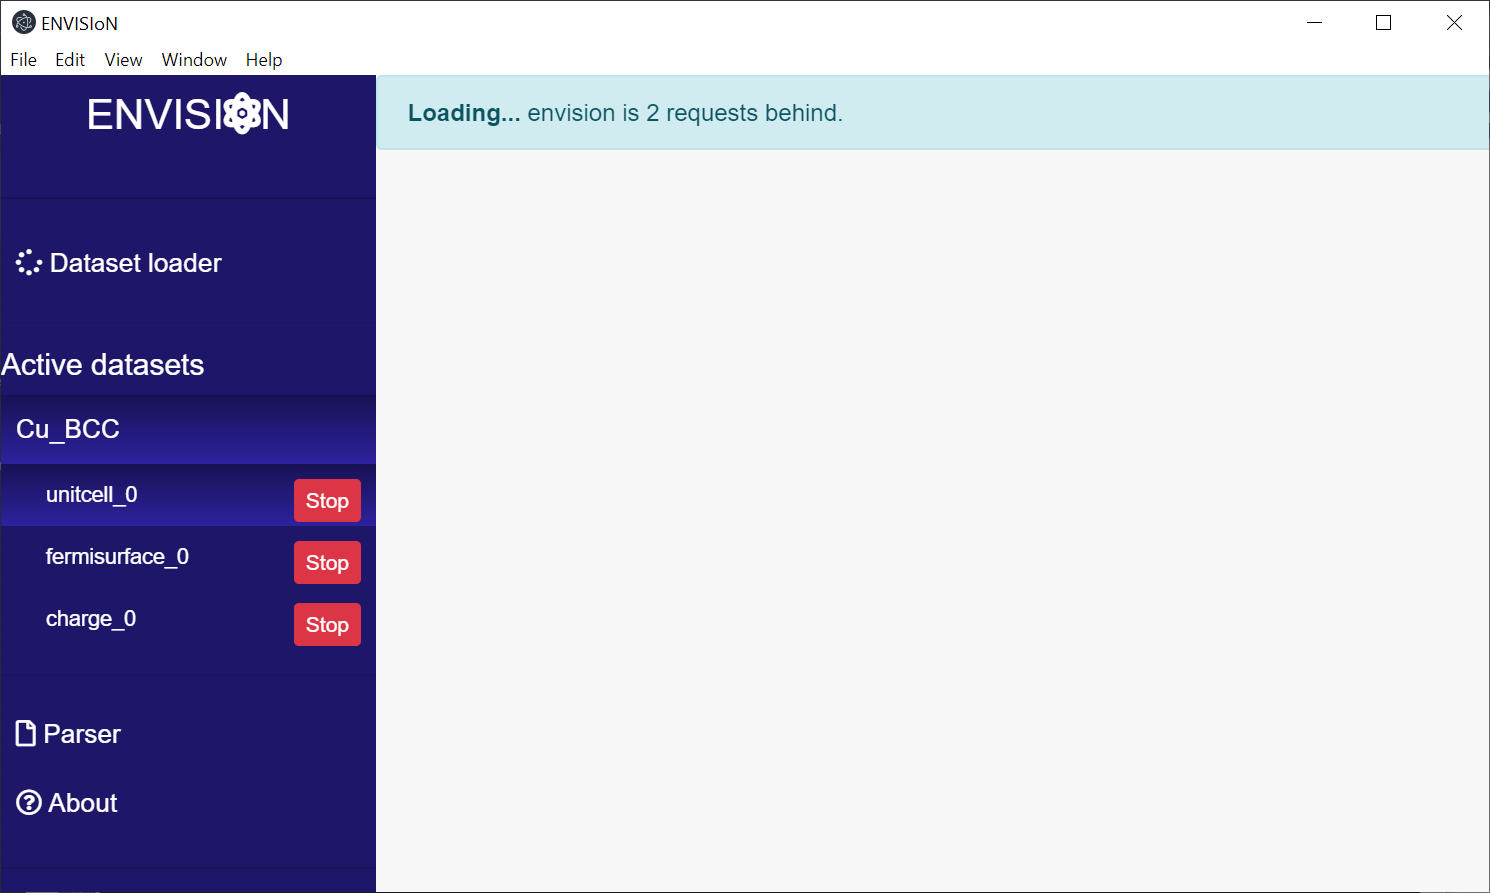
\includegraphics[scale = 0.45]{Images/EnvisionRequestsbehind.png}
    \caption{The pop up when ENVISIoN is a number of requests behind.}
    \label{fig:GUINotresponding}
\end{figure}

To recover from that ENVISIoN is a number of requests behind you can click on ``View'' in the upper menu and then ``Reload'' to reload the GUI. Then you need to start from the beginning and load the dataset once again.

If ENVISIoN is a number of request behind and the user continues to click around in the GUI and tries to load a new dataset or create a new visualisation the GUI will crash. If it does the following message box will pop up, see figure \ref{fig:GUIcrash}.

\begin{figure}[H]
    \centering
    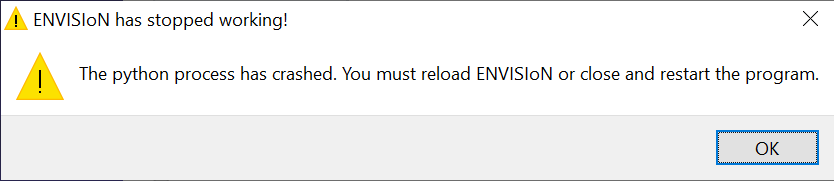
\includegraphics[scale = 0.55]{Images/Envisioncrashed.png}
    \caption{The message box when ENVISIoN crashes.}
    \label{fig:GUIcrash}
\end{figure}

To recover from that ENVISIoN crashes you can either reload the page as mentioned above, or just close the GUI window and restart ENVISIoN.

    \newpage
    \section{Common errors during installation}
\subsection{Qt}
Inviwo uses the graphics library Qt which isn't always installed properly. These instructions show how to download and install the latest version of Qt on Ubuntu 10.04 LTS. That is, in the moment of writing this user guide, version 5.12.3. 

To download the installation file into the \emph{~/Downloads} directory, simply execute the commands below.

\begin{lstlisting}[frame = single, breaklines=true]
    cd ~/Downloads
    wget http://download.qt.io/official_releases/qt/5.12/5.12.3/qt-opensource-linux-x64-5.12.3.run
    
    
    
\end{lstlisting}

When the installation file has finished downloading, the user won't have permission to run the file. To change permissions and run the file by executing the commands below and enter your superuser password immediately after.
\begin{lstlisting}[frame = single, breaklines=true]
    chmod +x qt-opensource-linux-x64-5.12.3.run
    sudo ./qt-opensource-linux-x64-5.12.3.run
\end{lstlisting}

An Qt installer is now shown on the screen. Notice that the manual installation will force a installation of the Qt editor as shown in step 6. The entire installation will occupy approximately 5.12 GB. Follow the instructions in figure \ref{fig:Qt} to complete the installation.

After the installation is done, the path to Qt needs to be added to the system. Add the necessary paths by executing the commands below.

\begin{lstlisting}[frame = single, breaklines=true]
    cd /usr/lib/x86_64-linux-gnu/qtchooser
    sudo echo "/opt/Qt5.12.3/5.12.3/gcc_64/bin" | sudo tee -a default.conf
    sudo echo "/opt/Qt5.12.3/5.12.3/gcc_64/lib" | sudo tee -a default.conf
\end{lstlisting}

The system is now ready for an Inviwo installation.

\begin{figure}[H]
    \centering
    \begin{subfigure}{0.32\linewidth}
        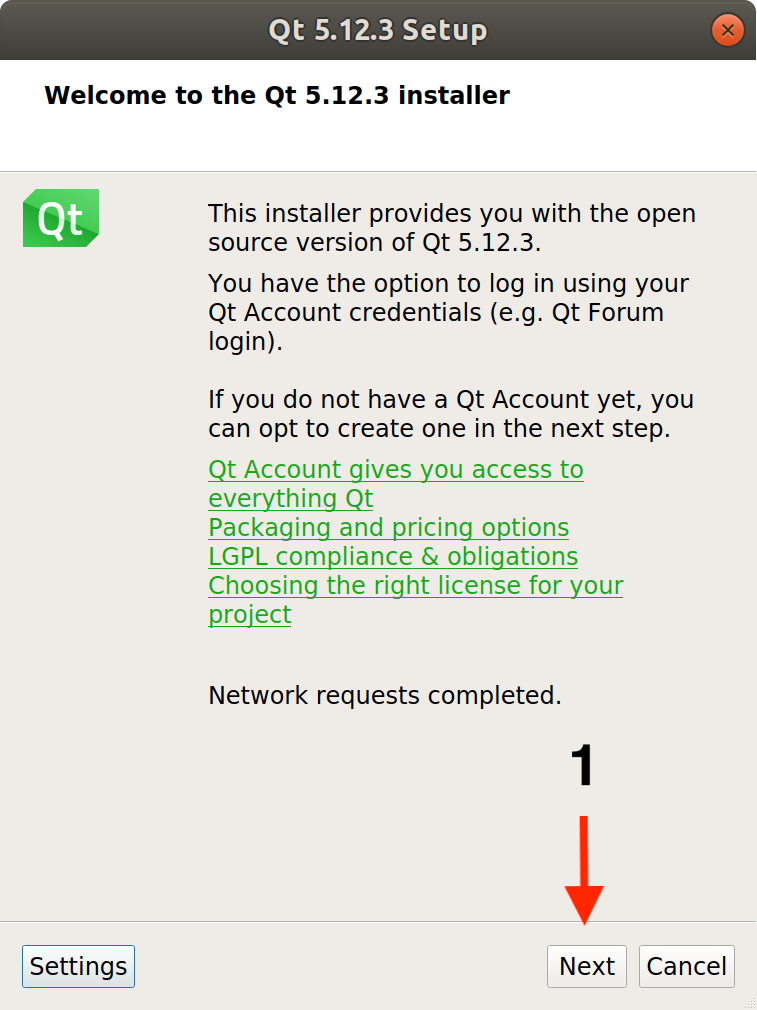
\includegraphics[width=1\textwidth]{images/Qt1.png}
    \end{subfigure}
    \begin{subfigure}{0.32\linewidth}
        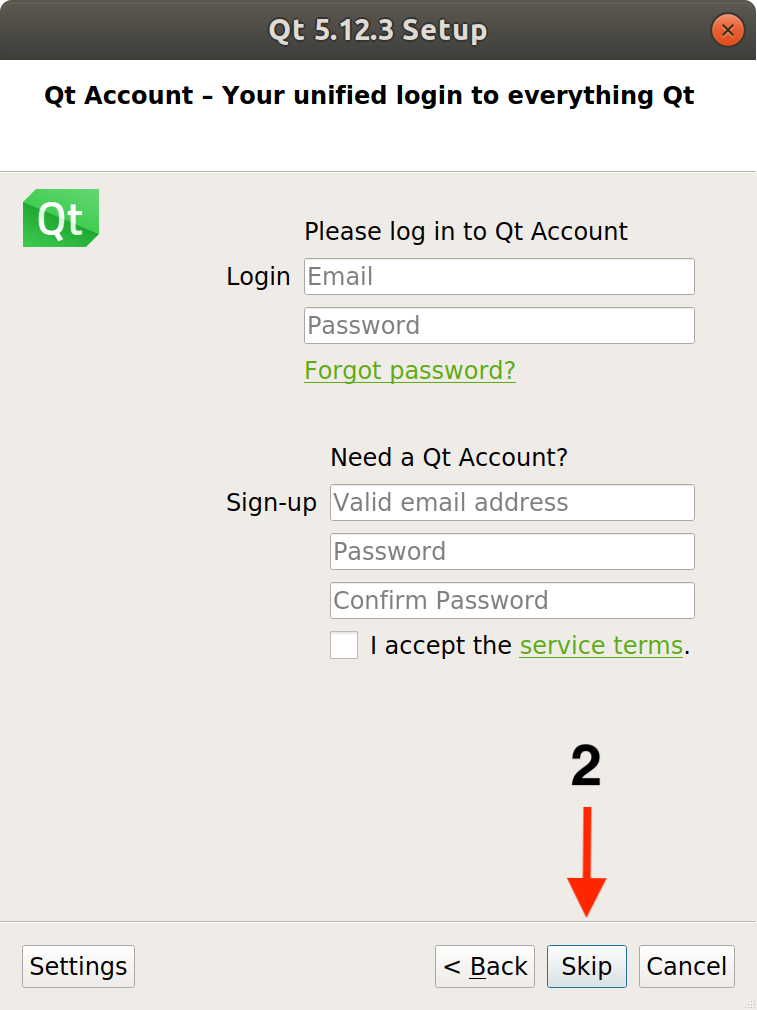
\includegraphics[width=1\textwidth]{images/Qt2.png}
    \end{subfigure}
    \begin{subfigure}{0.32\linewidth}
        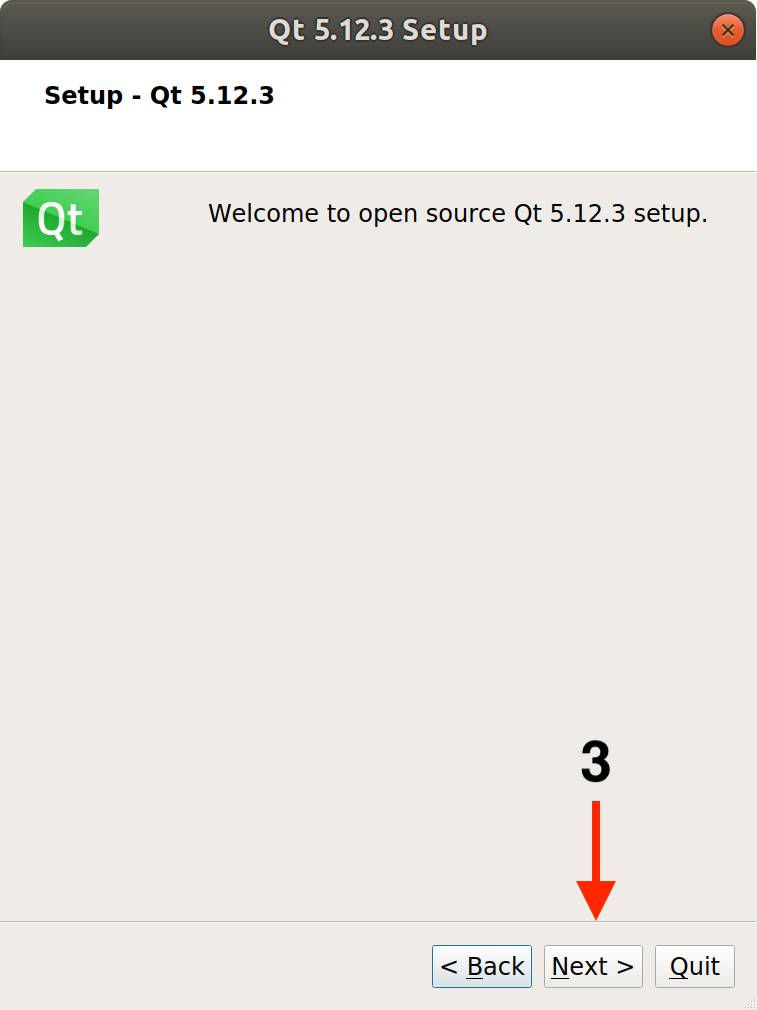
\includegraphics[width=1\textwidth]{images/Qt3.png}
    \end{subfigure}
    \begin{subfigure}{0.32\linewidth}
        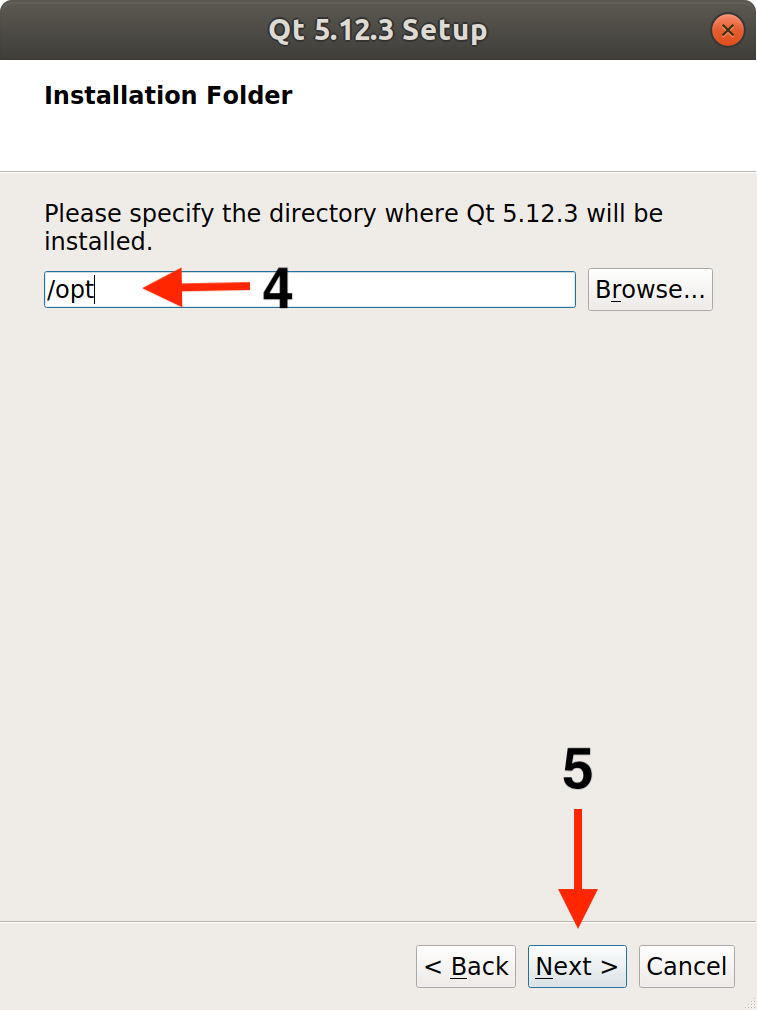
\includegraphics[width=1\textwidth]{images/Qt4.png}
    \end{subfigure}
    \begin{subfigure}{0.32\linewidth}
        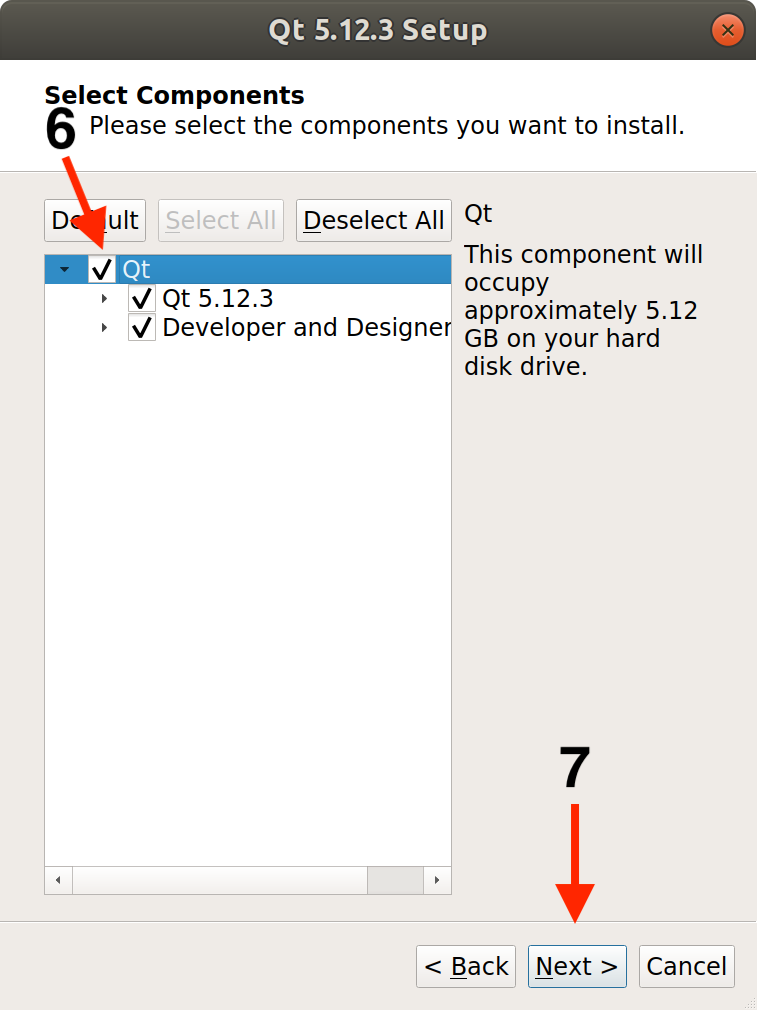
\includegraphics[width=1\textwidth]{images/Qt6.png}
    \end{subfigure}
    \begin{subfigure}{0.32\linewidth}
        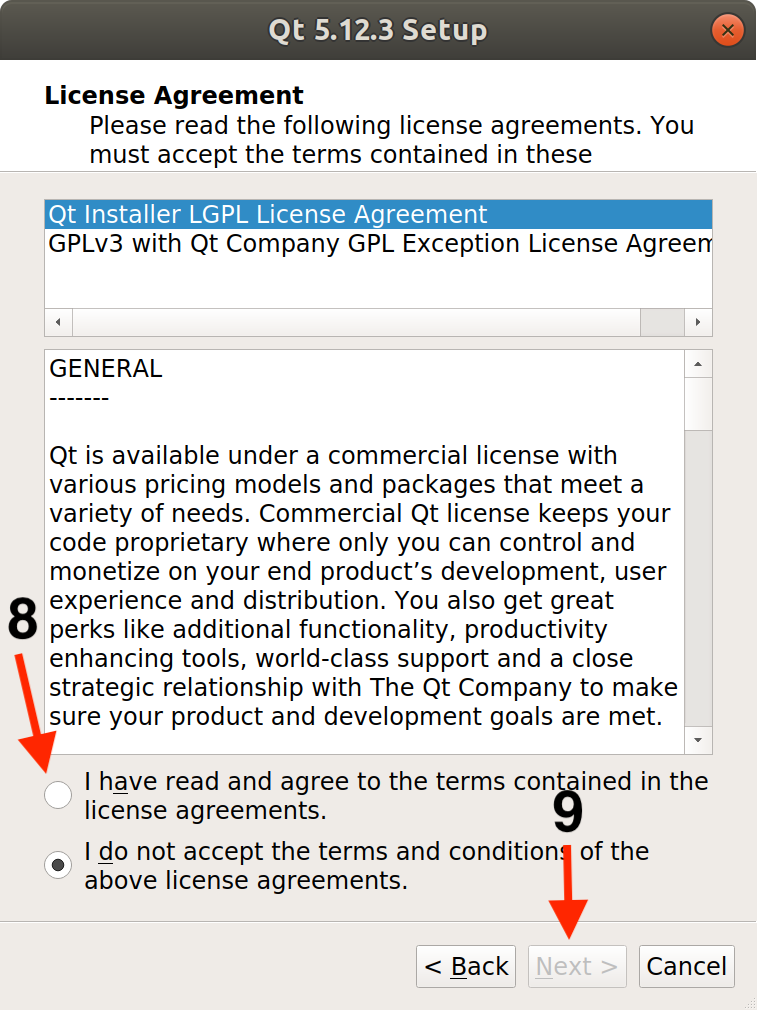
\includegraphics[width=1\textwidth]{images/Qt7.png}
    \end{subfigure}
    \begin{subfigure}{0.32\linewidth}
        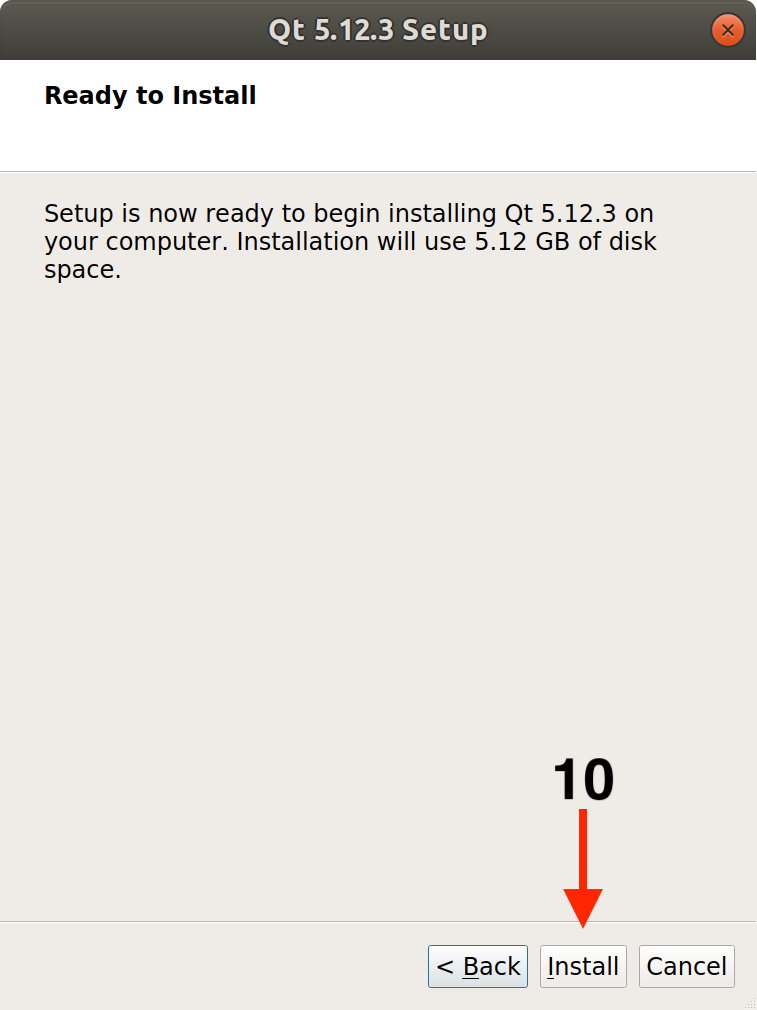
\includegraphics[width=1\textwidth]{images/Qt8.png}
    \end{subfigure}
    \caption{Instructions for installation of Qt 5.12.3.}
    \label{fig:Qt}
\end{figure}

    \newpage
    \printbibliography[title={References}, heading=bibintoc]
    \newpage
    \begin{appendices}
        \section{Licens}
\label{ref:licens}
Copyright (c) 2021: Gabriel Anderberg, Kristoffer Gubberud Maras, Adam Engman, Joakim Stenborg, Didrik Axén \newline \newline
Copyright (c) 2020: Alexander Vevstad, Amanda Aasa, Amanda Svennblad, Daniel Thomas, Lina Larsson, Olav Berg

Redistribution and use in source and binary forms, with or without
modification, are permitted provided that the following conditions are met:

\begin{enumerate}
    \item Redistributions of source code must retain the above copyright notice, this list of conditions and the following disclaimer.
    \item Redistributions in binary form must reproduce the above copyright notice, this list of conditions and the following disclaimer in the documentation and/or other materials provided with the distribution.
\end{enumerate}

THIS SOFTWARE IS PROVIDED BY THE COPYRIGHT HOLDERS AND CONTRIBUTORS "AS IS" AND ANY EXPRESS OR IMPLIED WARRANTIES, INCLUDING,
BUT NOT LIMITED TO, THE IMPLIED WARRANTIES OF MERCHANTABILITY AND FITNESS FOR A PARTICULAR PURPOSE ARE DISCLAIMED. IN NO EVENT
SHALL THE COPYRIGHT OWNER OR CONTRIBUTORS BE LIABLE FOR ANY DIRECT, INDIRECT, INCIDENTAL, SPECIAL, EXEMPLARY, OR CONSEQUENTIAL
DAMAGES (INCLUDING, BUT NOT LIMITED TO, PROCUREMENT OF SUBSTITUTE GOODS OR SERVICES; LOSS OF USE, DATA, OR PROFITS; OR BUSINESS
INTERRUPTION) HOWEVER CAUSED AND ON ANY THEORY OF LIABILITY, WHETHER IN CONTRACT, STRICT LIABILITY, OR TORT (INCLUDING
NEGLIGENCE OR OTHERWISE) ARISING IN ANY WAY OUT OF THE USE OF THIS SOFTWARE, EVEN IF ADVISED OF THE POSSIBILITY OF SUCH DAMAGE.

    \end{appendices}
\end{document}
